% Customizable fields and text areas start with % >> below.
% Lines starting with the comment character (%) are normally removed before release outside the collaboration, but not those comments ending lines

% svn info. These are modified by svn at checkout time.
% The last version of these macros found before the maketitle will be the one on the front page,
% so only the main file is tracked.
% Do not edit by hand!
\RCS$Revision: 226819 $
\RCS$HeadURL: svn+ssh://svn.cern.ch/reps/tdr2/papers/SMP-13-009/trunk/SMP-13-009.tex $
\RCS$Id: SMP-13-009.tex 226819 2014-02-10 20:22:04Z jdamgov $
%%%%%%%%%%%%% local definitions %%%%%%%%%%%%%%%%%%%%%
% This allows for switching between one column and two column (cms@external) layouts
% The widths should  be modified for your particular figures. You'll need additional copies if you have more than one standard figure size.
\newlength\cmsFigWidth
\ifthenelse{\boolean{cms@external}}{\setlength\cmsFigWidth{0.85\columnwidth}}{\setlength\cmsFigWidth{0.4\textwidth}}
\ifthenelse{\boolean{cms@external}}{\providecommand{\cmsLeft}{top}}{\providecommand{\cmsLeft}{left}}
\ifthenelse{\boolean{cms@external}}{\providecommand{\cmsRight}{bottom}}{\providecommand{\cmsRight}{right}}
%%%%%%%%%%%%%%%  Title page %%%%%%%%%%%%%%%%%%%%%%%%
\cmsNoteHeader{SMP-13-009} % This is over-written in the CMS environment: useful as preprint no. for export versions
\newcommand{\mjj}{\ensuremath{m_{jj}}}%
\renewcommand{\MET}{\ensuremath{{E\!\!\!/}_{\!\mathrm{T}}}\xspace}
% >> Title: please make sure that the non-TeX equivalent is in PDFTitle below
\title{A search for $WW\gamma$ and $WZ\gamma$ production and anomalous quartic gauge couplings in pp collisions at 
$\sqrt{s}$ = 8 TeV}

% >> Authors
%Author is always "The CMS Collaboration" for PAS and papers, so author, etc, below will be ignored in those cases
%For multiple affiliations, create an address entry for the combination
%To mark authors as primary, use the \author* form
%% \address[neu]{Northeastern University}
%% \address[fnal]{Fermilab}
%% \address[cern]{CERN}
\author[cern]{The CMS Collaboration}

% >> Date
% The date is in yyyy/mm/dd format. Today has been
% redefined to match, but if the date needs to be fixed, please write it in this fashion.
% For papers and PAS, \today is taken as the date the head file (this one) was last modified according to svn: see the RCS Id string above.
% For the final version it is best to "touch" the head file to make sure it has the latest date.
\date{\today}

% >> Abstract
% Abstract processing:
% 1. **DO NOT use \include or \input** to include the abstract: our abstract extractor will not search through other files than this one.
% 2. **DO NOT use %**                  to comment out sections of the abstract: the extractor will still grab those lines (and they won't be comments any longer!).
% 3. **DO NOT use tex macros**         in the abstract: External TeX parsers used on the abstract don't understand them.
\abstract{
   A study of the WV$\gamma$ triple vector boson production is presented 
   based on events containing a W boson decaying to an muon or a electron and a neutrino,
   a second V (W or Z) boson decaying to two jets, and a photon.
   The dataset corresponds to an integrated luminosity of 19.3~fb$^{-1}$
   collected in 2012 with the CMS detector at the LHC in pp collisions at $\sqrt{s}$ = 8~TeV.
   The cross section is estimated for a final state with photon transverse energy
   above 30 GeV and with an absolute value of pseudorapidity of less than 1.44. 
   An upper limit of 311 fb on the cross section for standard model production of the WV$\gamma$ process is obtained at 95\% 
   confidence level. This is approximately a factor of 3.4 larger than the predictions from next-to-leading order
   QCD calculations. No evidence of anomalous WW$\gamma\gamma$ or WWZ$\gamma$ quartic gauge boson couplings is found.
   This paper presents the first experimental limits on the dimension 8 WW$\gamma\gamma$ parameter
   $f_{T,0}$ and the CP-conserving WWZ$\gamma$ parameters $\kappa_0^W$ and $\kappa_C^W$. Competitive
   limits are also obtained for the WW$\gamma\gamma$ parameters $a_{0}^{W}$ and $a_{C}^{W}$.
}

% >> PDF Metadata
% Do not comment out the following hypersetup lines (metadata). They will disappear in NODRAFT mode and are needed by CDS.
% Also: make sure that the values of the metadata items are sensible and are in plain text:
% (1) no TeX! -- for \sqrt{s} use sqrt(s) -- this will show with extra quote marks in the draft version but is okay).
% (2) no %.
% (3) No curly braces {}.
\hypersetup{%
pdfauthor={WWA team},%
pdftitle={A Search for WWgamma and WZgamma production in pp Collisions at sqrt(s) = 8 TeV.},%
pdfsubject={CMS},%
pdfkeywords={CMS, physics, software, computing}}

\maketitle %maketitle comes after all the front information has been supplied
% >> Text
%%%%%%%%%%%%%%%%%%%%%%%%%%%%%%%%  Begin text %%%%%%%%%%%%%%%%%%%%%%%%%%%%%
%% **DO NOT REMOVE THE BIBLIOGRAPHY** which is located before the appendix.
%% You can take the text between here and the bibiliography as an example which you should replace with the actual text of your document.
%% If you include other TeX files, be sure to use "\input{filename}" rather than "\input filename".
%% The latter works for you, but our parser looks for the braces and will break when uploading the document.
%%%%%%%%%%%%%%%
%\tableofcontents
\newpage

In the present iteration of the analysis our goal is to 
reconstruct either a linear discriminant or likelihood of 
minimum number of uncorrelated variables necessary to 
describe the event topology. 
This is because the individual cuts are highly 
inefficient. 
To keep the analysis as simple as possible we have intentionally 
not focused on exploiting the full potential of the 
multivariate analysis because this would involve 
inclusion of additional correlated variables.



\subsection{Training and validation method}
The Toolkit for Multivariate Data Analysis with ROOT 
(TMVA)~\cite{tmva}
is a toolkit to be implemented using ROOT that allows the user 
to carry out a significant number of multivariate analysis 
techniques such as boosted decision trees, neural networks, 
projected likelihood estimators and linear discriminants.

Using TMVA to implement the majority of these techniques 
consists of two phases: the Training Phase and the Testing Phase. 
To begin the Training Phase, the user must have samples where 
it is known which events are to be classified as signal and which 
are to be classified as background. 
Using this information, TMVA is trained to separate these classes 
as efficiently as possible. 
Next, the Testing Phase simply stands to implement the trained 
method of separation on a dataset where it is unknown which 
events are to be classified as signal or background. 

In the present analysis we try three classifiers to separate 
Higgs signal from the background: linear discriminant (LD),
likelihood, and boosted decision tree (BDT).
We have tried to use a complete set of minimum number of 
input variables necessary to describe the whole event topology, 
as will be described in detail in the next section.


The TMVA has some knobs to optimize the
performance of various classifiers, but we didn't tune these knobs. 
In the region of interest to us (90--95\% background
rejection points) the likelihood and BDT classifiers have almost 
identical performance. 
This is expected because the input variables are mostly uncorrelated, 
and there are no large correlations to be exploited.

We have also seen in the previous iterations of training that
with inclusion of additional (correlated) variables the BDT
performs better than likelihood. However, some of these
variables were correlated with the 4-body mass ($m_{WW} = m_{\ell\nu jj}$), 
so we decided to trim down to the minimum possible complete
set comprising of 10 variables. 


\subsection{Training and validation samples}
We perform a two-component multivariate analysis (MVA) to 
separate the Higgs signal from the dominant W+jets background.
We used the Fall11 MC samples for both Higgs signal and the 
W+jets background, as listed in Table~\ref{tab:MCsamples}.
%%%%%%%%%%%%%%%%%%%%%%%%%%
\begin{table}[htb]
  \begin{center}
    \begin{tabular}{l|l} 
      \hline
       Category & Sample name\\
      \hline
      Background & {\footnotesize /WJetsToLNu\_TuneZ2\_7TeV-madgraph-tauola/Fall11-PU\_S6\_START42\_V14B-v1/AODSIM}  \\
      \hline
      Signal &  {\footnotesize /GluGluToHToWWToLNuQQ\_M-*\_7TeV-powheg-pythia6/Fall11-PU\_S6\_START42\_}\\
       &  {\footnotesize V14B-v1/AODSIM} (with Higgs mass from 170 to 600~GeV) \\
      \hline
    \end{tabular}
  \end{center}
  \caption{Summary of Monte Carlo training and testing samples used in the analysis. 
    We use 50\% of the events in each category for training and the other 50\% for testing/validation.}
  \label{tab:MCsamples}
\end{table}
%%%%%%%%%%%%%%%%%%%%%%%%%%

\subsection{Training method}
We train the MVA separately for the following 12 Higgs mass 
points: 170, 180, 190, 200, 250, 300, 350, 400, 450, 500, 550, and 600~GeV.
Exactly 50\% of the events in each category are used for training 
the classifier and the other 50\% are used for testing/validation.
We train separately the events with two jets 
and three jets in the final state, because the background composition 
and kinematics are different for the two categories.
We also train separately for the two lepton species, \textit{i.e.}, 
muons and electrons.
In the following sections we will show the plots for muon channel 
only because the corresponding plots for the electron channel are 
very similar.


\subsection{Selection cuts}
Selection cuts are identical to the pre-selection described in 
CMS AN-2011/110. These include requirements on lepton ID, loose 
jet ID, second lepton veto in the event, and minimum missing transverse 
energy (25 GeV for muon and 35 GeV for electron events). 


%\clearpage{}
\section{Theoretical framework}
\label{sec:aQGCth}

An effective field theory approach is adopted in which
higher-dimensional operators supplement the SM Lagrangian to include anomalous gauge coumpings, as discussed
in Refs. ~\cite{Eboli:2006wa,Belanger:1999,Bosonic:2004PRD}. Within this
framework, anomalous boson interactions can be parametrized using two
possible realizations. The first is a nonlinear realization of the
$SU(2)\otimes U(1)$ gauge symmetry, which is broken by means other
than the conventional Higgs scalar doublet. The quartic boson
interactions involving photons appear as dimension 6 operators. The
second is a linear realization of the symmetry, which is broken by the
conventional Higgs scalar doublet field. The quartic interactions
involving photons appear as dimension 8 operators. 

Some of the operators within the two realizations share similar Lorentz structures,
which means that their parameters can therefore be expressed simply in
terms of parameters from the other realization, whereas others
cannot. The inclusion of such higher-dimensional operators causes the
theory to violate unitarity, unless one adopts a form factor to avoid
unphysical behavior of the cross section. While the discovery of the SM Higgs boson makes the linear realization
more appropriate for AQGC searches~\cite{Aihara:1995iq,Baak:2013fwa},
there are a total of 14 such operators that can contribute to the
anomalous coupling signal. In addition, all published AQGC limits to
date are expressed in terms of dimension 6 parameters. To bridge this
divide, we select four dimension 6 parameters, two of which have not
been previously measured, and the other two are used to compare with
previous results~\cite{Belanger:1999,Achard:2001eg}. These parameters
also have dimension 8 analogues. Finally, we include a representative
parameter from the linear realization, $f_{T,0}$, which has no
dimension 6 analogue.

The Feynman diagrams for the quartic vertices are shown in
Figure~\ref{fig:feyndiag}, and the CP-conserving, anomalous
interaction Lagrangian terms chosen for this analysis are shown in
Eq.~\eqref{lagrangian}.

\begin{figure}[htb]
  \begin{center}
  \scalebox{0.90}{
%    \subfigure[]{
      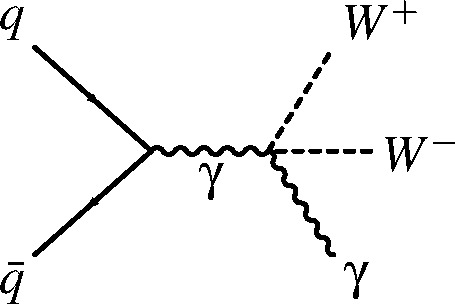
\includegraphics[width=0.35\textwidth]{figs/wwaa.pdf}
%    }
    \hspace{1cm}
%    \subfigure[]{
      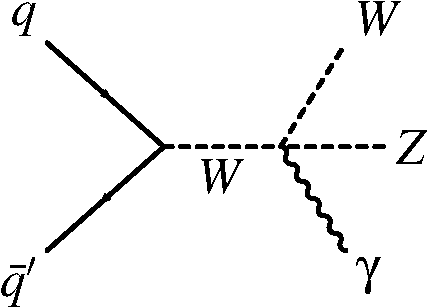
\includegraphics[width=0.35\textwidth]{figs/wwza.pdf}
%    }
}

    \caption{Feynman diagrams that involve a quartic vector boson vertex. Both diagrams are present in the SM.}
    \label{fig:feyndiag}
  \end{center}
\end{figure} 


\begin{eqnarray}\label{lagrangian}
{\cal L}_{\textrm{AQGC}} &=& -\dfrac{e^2}{8} \dfrac{a_0^W}{\Lambda^2} F_{\mu \nu} F^{\mu \nu} W^{+\alpha} W^-_{\alpha} - \dfrac{e^2}{16} 
\dfrac{a_C^W}{\Lambda^2} F_{\mu \nu} F^{\mu \alpha} ( W^{+\nu} W^-_{\alpha} + W^{-\nu} W^+_{\alpha} ) \nonumber \\
& &- e^2 g^2 \dfrac{\kappa_0^{W}}{\Lambda^2} F_{\mu \nu} Z^{\mu \nu} W^{+ \alpha} W^-_{\alpha}- \frac{e^2 g^2}{2} \dfrac{\kappa_C^{W}}{\Lambda^2} F_{\mu \nu} Z^{\mu \alpha} ( W^{+\nu} W^-_{\alpha} + W^{-\nu} W^+_{\alpha} )\nonumber \\ 
& &+ \dfrac{f_{T,0}}{\Lambda^4} Tr[\hat{W}_{\mu \nu} \hat{W}^{\mu \nu}] \times Tr[\hat{W}_{\alpha \beta} \hat{W}^{\alpha \beta}] .
\end{eqnarray}

The dimension 6 parameters $a_0^W/\Lambda^2$ and $a_C^W/\Lambda^2$ are
associated with the WW$\gamma\gamma$ vertex and the
$\kappa_0^W/\Lambda^2$ and $\kappa_C^W/\Lambda^2$ parameters are
associated with the WWZ$\gamma$ vertex. The dimension 8 parameter
$f_{T,0}/\Lambda^4$ contributes to both vertices. The
$a_{0,C}^W/\Lambda^2$ coupling parameters~\cite{Belanger:1999} have
dimension 8 analogues, the $f_{M,i}/\Lambda^4$ coupling parameters. The relationship between the two is as follows:

\begin{center}
\begin{eqnarray}
\dfrac{a_0^W}{\Lambda^2} &= &-\dfrac{4 M_W^2}{g^2} \dfrac{f_{M,0}}{\Lambda^{ 4}} - \dfrac{8 M_W^2}{g^{' 2}} \dfrac{f_{M,2}}{\Lambda^{ 4}}, \nonumber \\ 
\dfrac{a_C^W}{\Lambda^2} &= &\dfrac{4 M_W^2}{g^2} \dfrac{f_{M,1}}{\Lambda^{ 4}} + \dfrac{8 M_W^2}{g^{' 2}} \dfrac{f_{M,3}}{\Lambda^{ 4}},
\label{dim6to8}
\end{eqnarray}
\end{center}
where $g = e/\sin(\theta_W), g^{'} = e/\cos(\theta_W)$, $\theta_W$ is
the Weinberg angle, $e$ is the unit of electric charge, and $\Lambda$
represents the energy scale of possible new physics represented by these operators. 
%The validity of the expressions listed in Eq.~\eqref{dim6to8} are
%checked using numerical simulations, as shown in Figure~\ref{fig:dim6dim8trans}. 
The expressions listed in Eq.~\eqref{dim6to8} are used to translate 
the AQGC limits obtained for $a_{0,C}^W/\Lambda^2$, into limits on $f_{M,i}/\Lambda^4$.

%% \begin{figure}[htb]
%% \begin{center}
%%    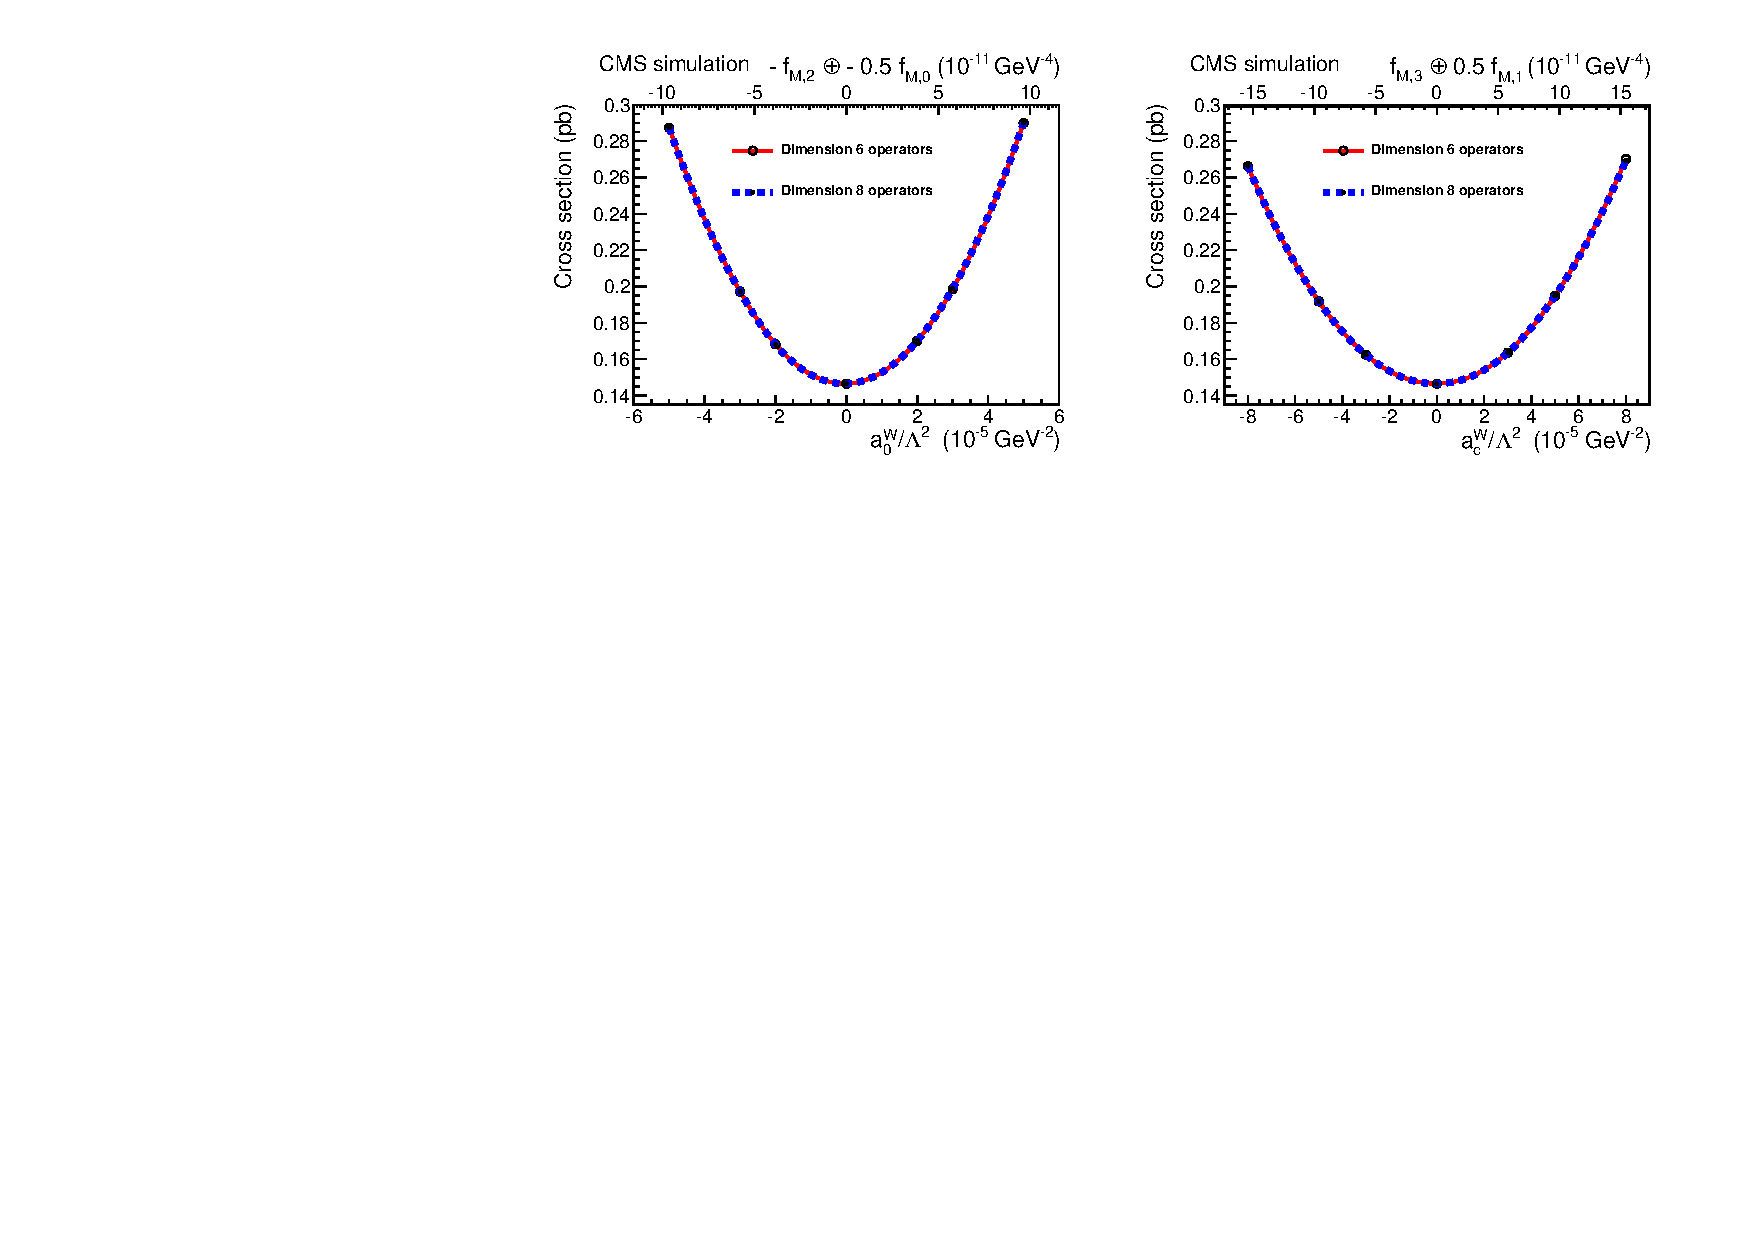
\includegraphics[width=.9\textwidth]{figs/comp628.pdf}
%% \caption{Predictions of the cross section as a function of the dimension 8 parameters $f_{M,i}$ and dimension 6 parameters $a_{0}^W$ and $a_{C}^W$.}
%% \label{fig:dim6dim8trans}
%% \end{center}
%% \end{figure}

Any nonzero value of the AQGCs will lead to tree-level unitarity
violation at sufficiently high energy. Therefore we calculated the
unitarity bounds \cite{Chapon:2009,AQGC:2001} for each AQGC parameter
as a function of $\Lambda_{ff}$ and $\hat{s}$ and substituted in a
dipole form factor $\alpha\rightarrow\frac{\alpha}{(1 +
\hat{s}/\Lambda_{ff}^2)^2}$, where $\alpha$ is an AQGC parameter,
$\Lambda_{ff}$ is the form factor scale and $\sqrt{\hat{s}}$ is the
center-of-mass energy of the interacting partons.  Illustration of the
unitarity bound and the expected limits are shown in Figure
\ref{fig:unitarity} for $a_{0}^{W}/\Lambda^{2}$,
$a_{C}^{W}/\Lambda^{2}$, and $f_{T,0}/\Lambda^{4}$, as a function of
$\Lambda_{ff}$.  The typical value for $\sqrt{\hat{s}}$ is 2~TeV for
values of the AQGC parameters close to the expected
limits~(Section \ref{sec:limits_pT}).

Figure~\ref{fig:unitarity} indicates that the effective field theory
terms directly violate unitarity at parameter values close to the
expected limits, and that the unitarity condition cannot be generally
satisfied for any scale $\Lambda_{ff}$ by the addition of such a form
factor. However, unitarity conserving new physics with a structure
more complex than that represented by a dipole form factor is
possible, making this search directly sensitive to new physics.  Since
the structure of such new physics is not known \textit{a priori}, the
choice is made to set limits without using form factors.  
%At 14 TeV, with larger data sets, these searches will also be directly sensitive
%to new physics that can be represented by an effective field theory.


\begin{figure}[hb]
  \begin{center}
    \subfigure[]{
    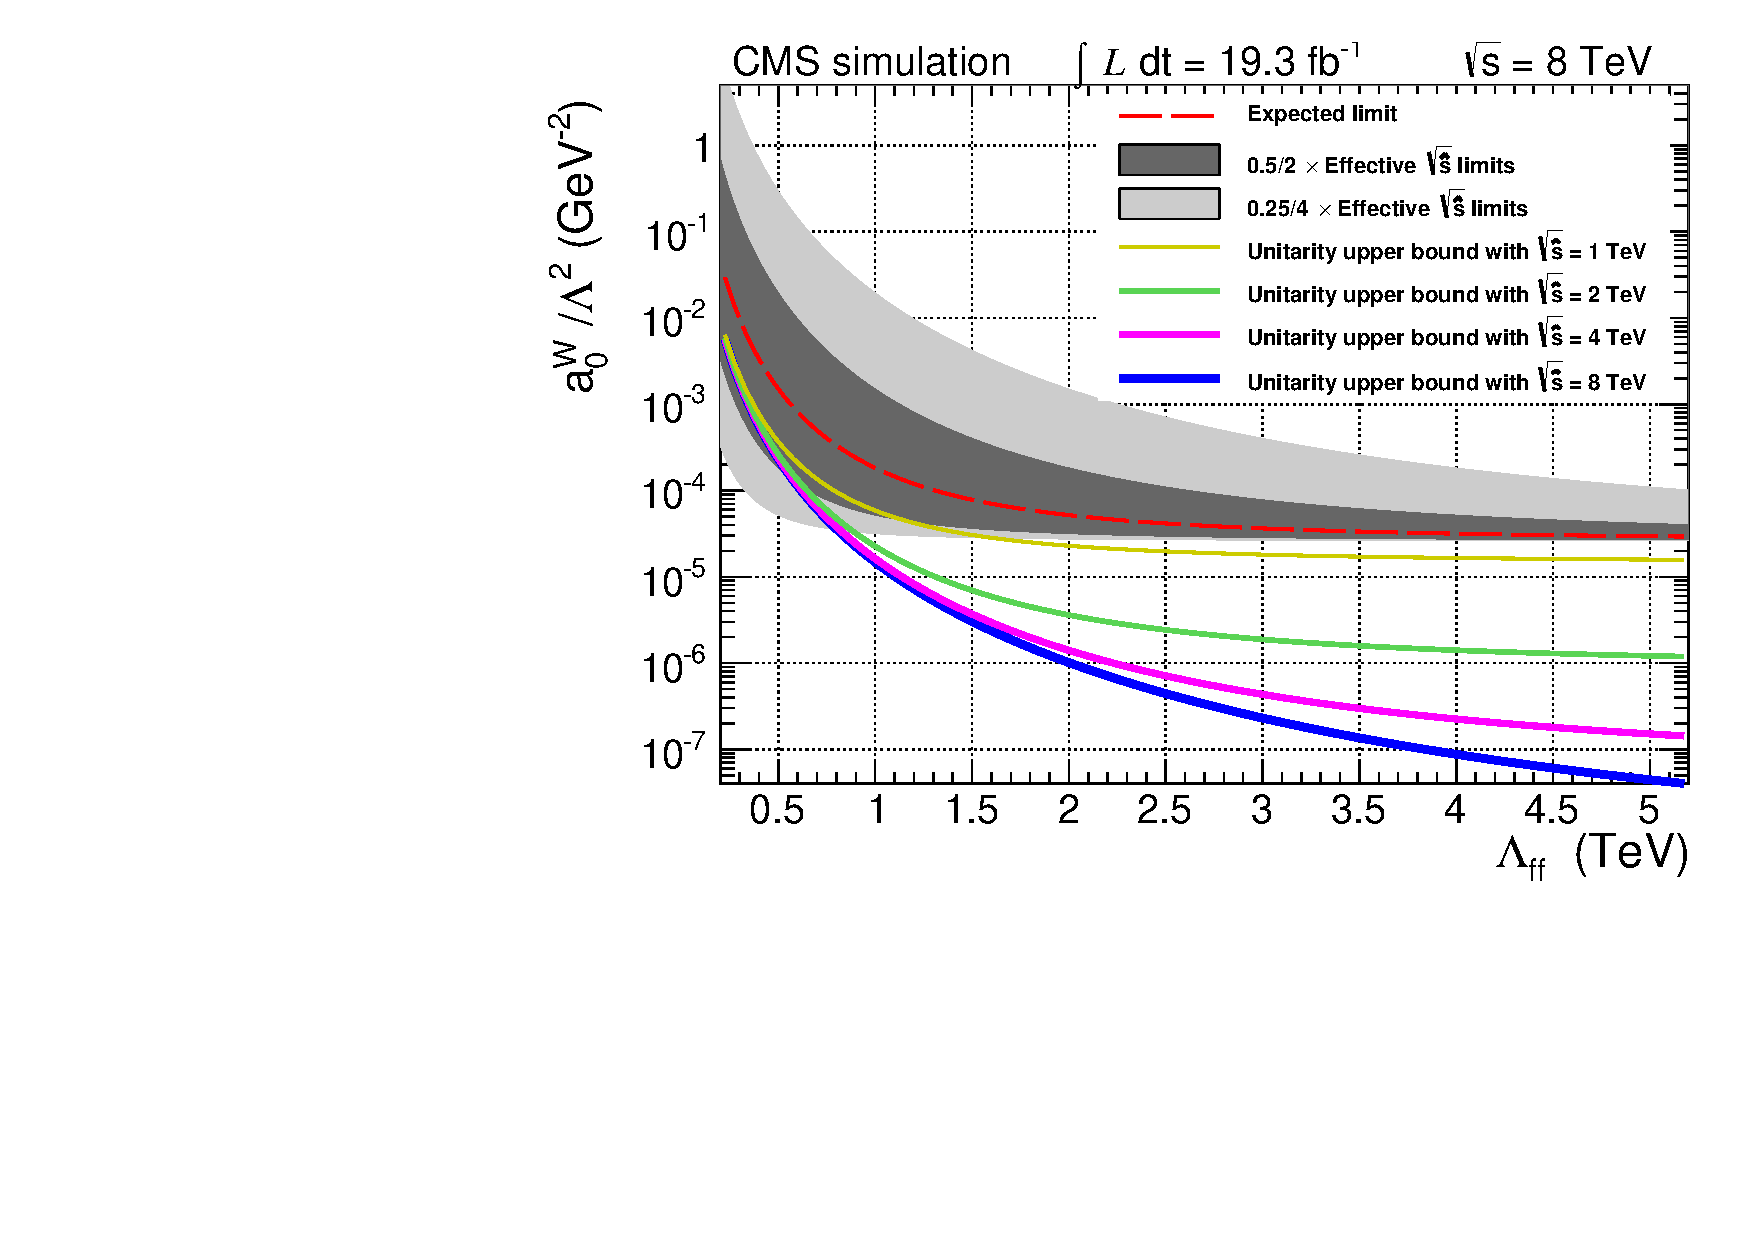
\includegraphics[width=0.51\textwidth]{figs/prounitarity_a0w.pdf}
  }
    \subfigure[]{
    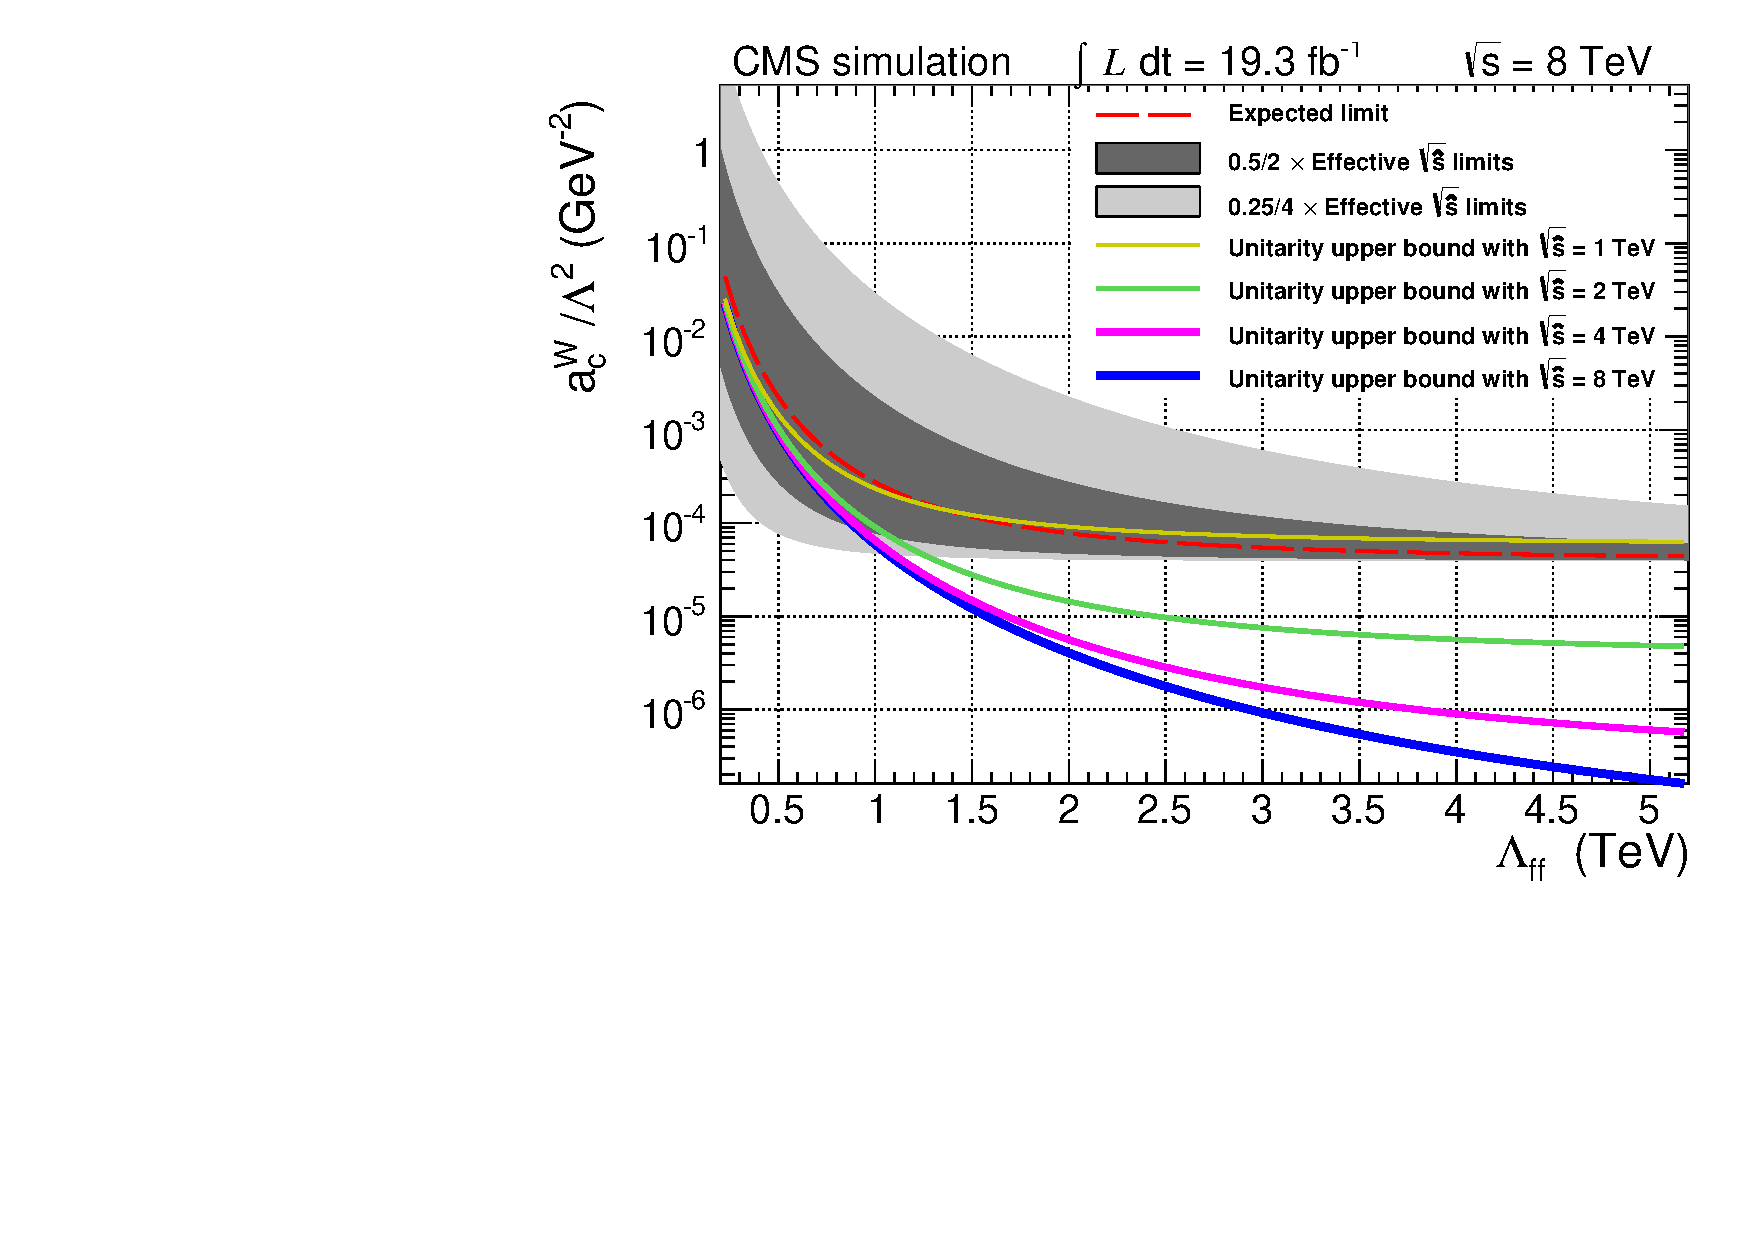
\includegraphics[width=0.51\textwidth]{figs/prounitarity_acw.pdf}
  }\\
  \subfigure[]{
    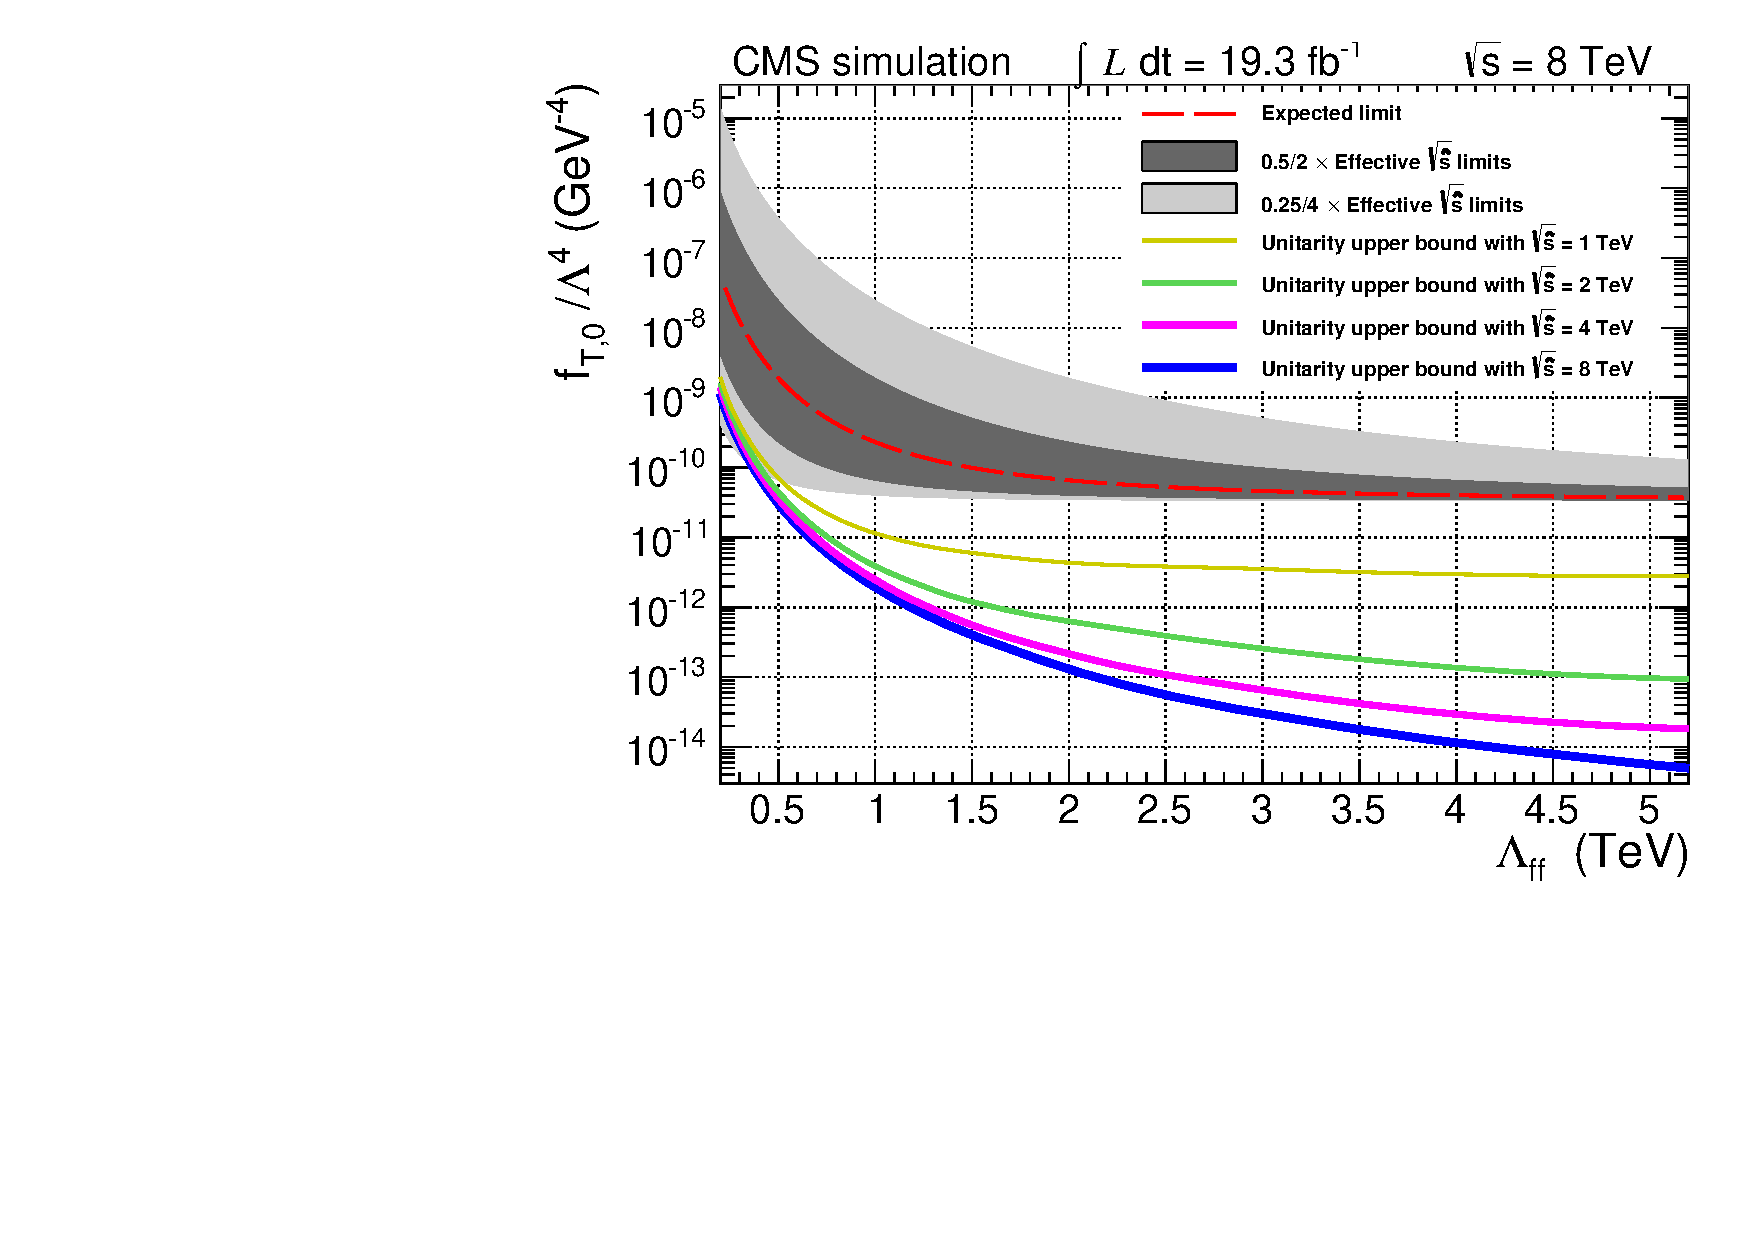
\includegraphics[width=0.51\textwidth]{figs/prounitarity_fT0.pdf}
  }
  \subfigure[]{
    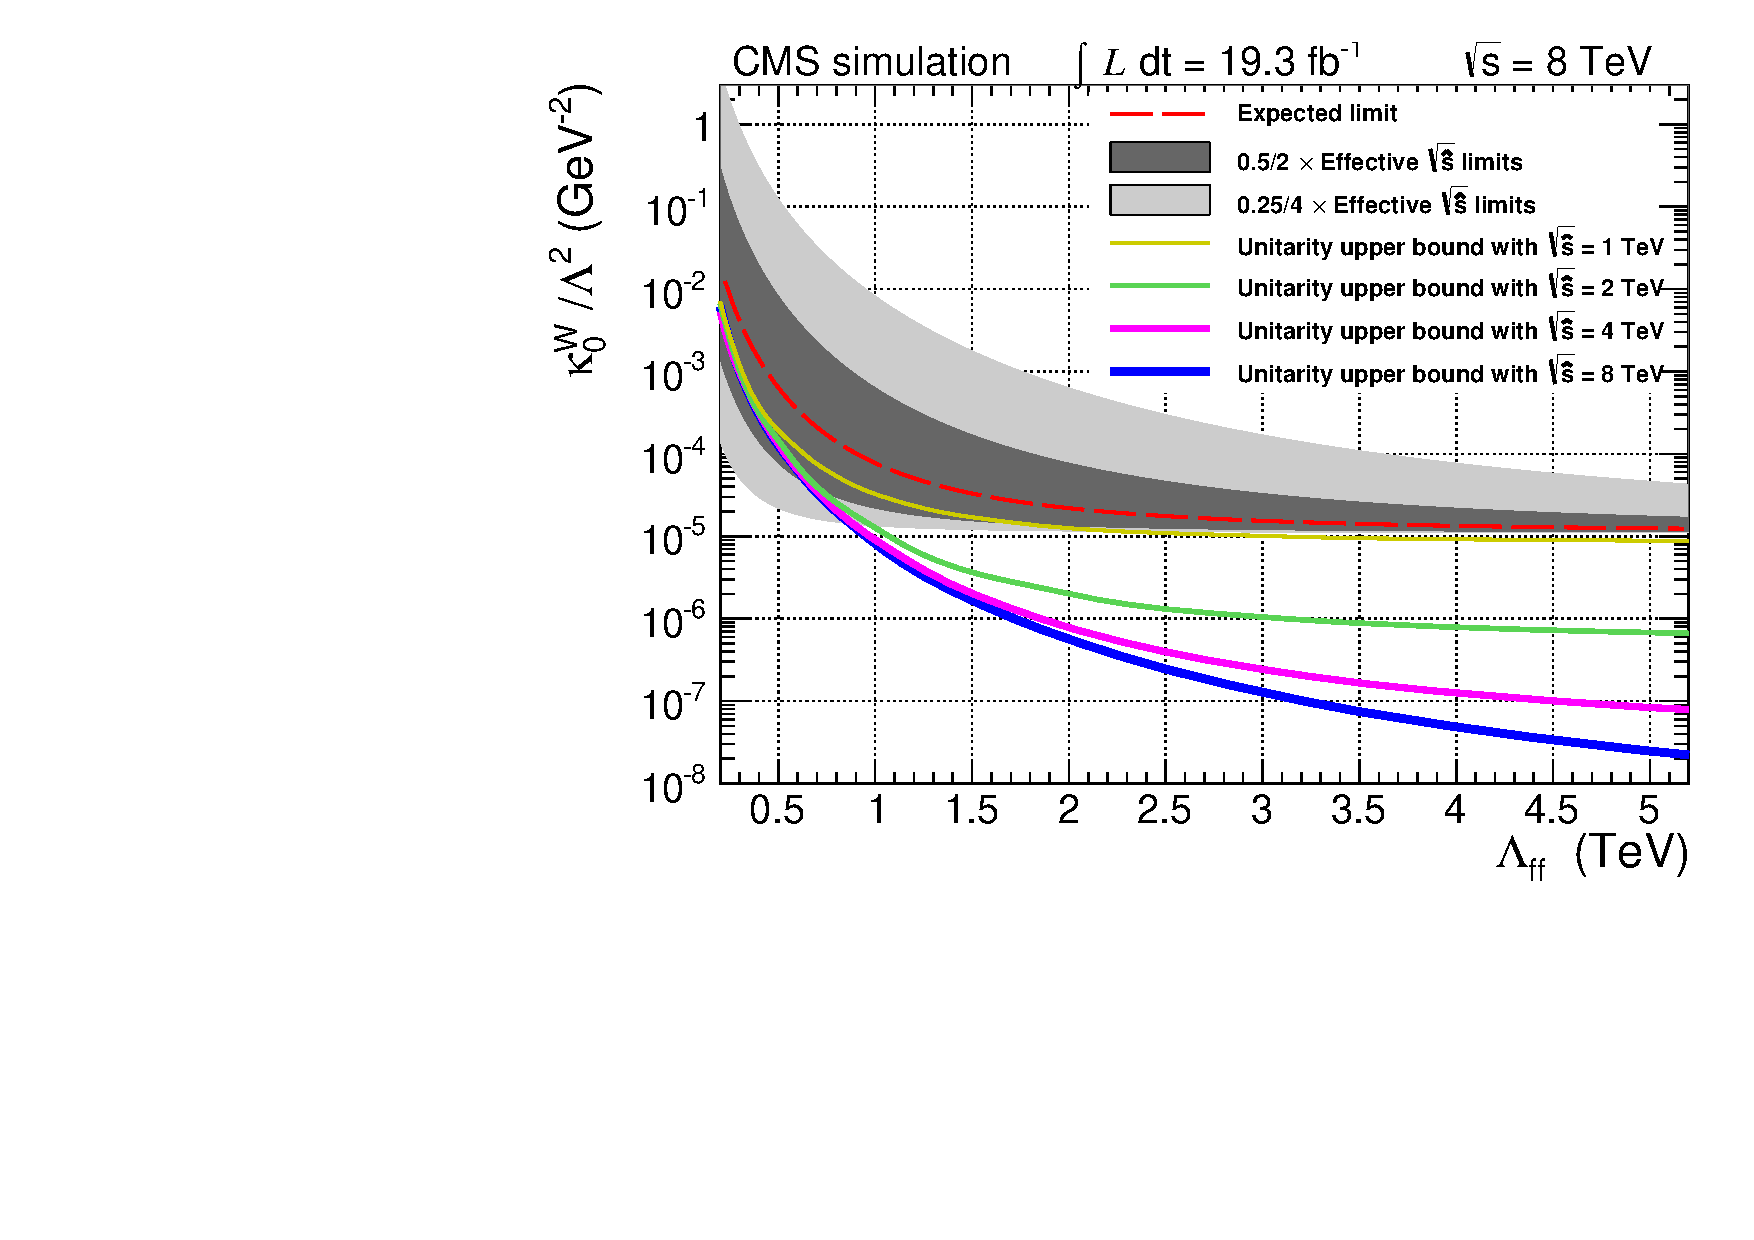
\includegraphics[width=0.51\textwidth]{figs/prounitarity_k0W.pdf}
  } \\
  \subfigure[]{
    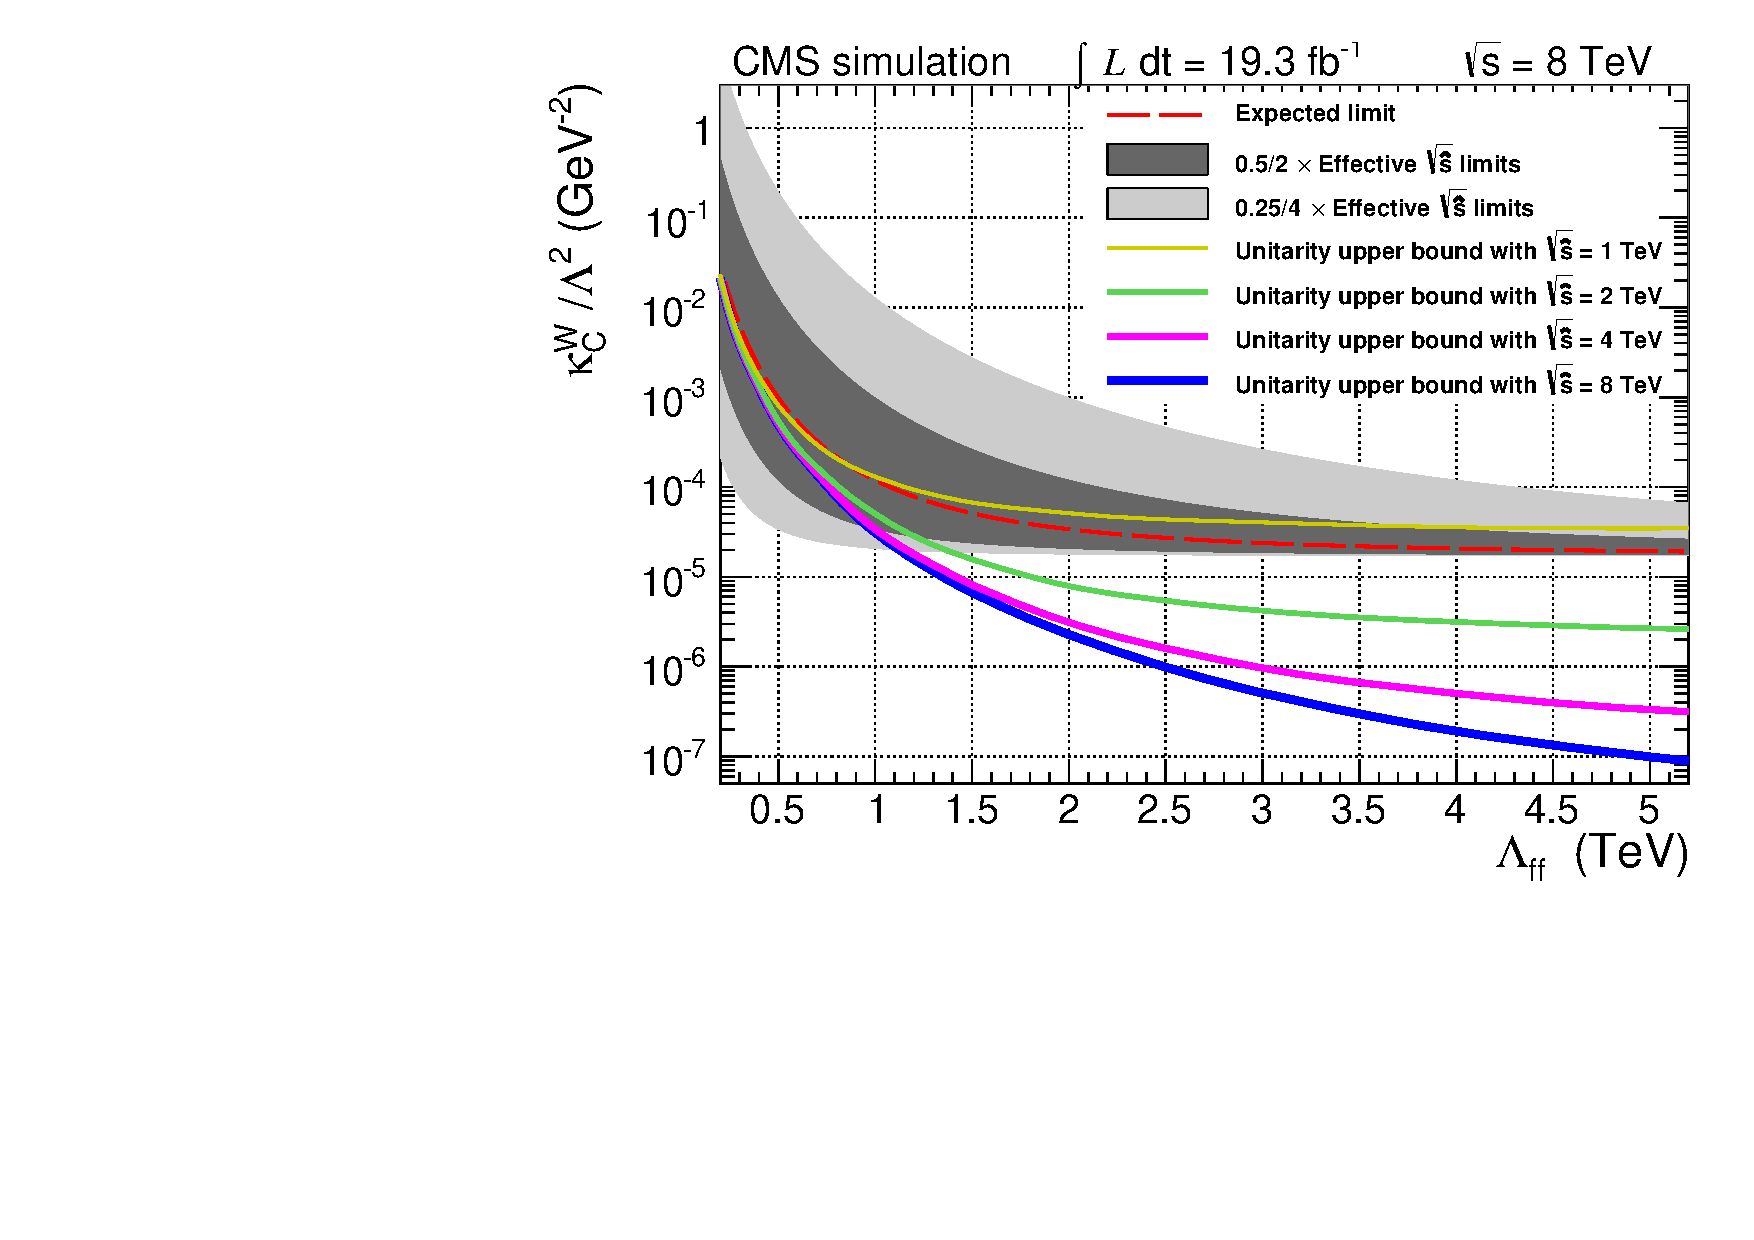
\includegraphics[width=0.51\textwidth]{figs/prounitarity_kCW.pdf}
  }
    \caption{ Unitarity bound as a function of the dipole form factor
scale $\Lambda_{ff}$ for (a) $a_{0}^{W}/\Lambda^{2}$, (b)
$a_{C}^{W}/\Lambda^{2}$, (c) $f_{T,0}/\Lambda^{4}$, (d)
$\kappa_{0}^{W}/\Lambda^{2}$, and (e) $\kappa_{C}^{W}/\Lambda^{2}$.
The dashed red lines represent the expected limits of this analysis,
and the gray bands represent regions around the expected limits with
$\hat{s}$ varied by a factor of 2 or 4. The colored curves represent
the unitarity bounds for fixed values of $\hat{s}$, above which
unitarity is violated.}
    \label{fig:unitarity}
  \end{center} \end{figure}


\section{The CMS detector }
\label{sec:CMSdet}

The central feature of the Compact Muon Solenoid (CMS) apparatus is a
superconducting solenoid of 6\unit{m} internal diameter and 13\unit{m} length, providing a
magnetic field of 3.8\unit{T}. Within the superconducting solenoid
volume are a silicon pixel and strip tracker, a lead tungstate crystal
electromagnetic calorimeter (ECAL), and a brass/scintillator hadron
calorimeter (HCAL). Muons are reconstructed in gas-ionization detectors
embedded in the steel flux return yoke outside the solenoid. Extensive
forward calorimetry complements the coverage provided by the barrel
and endcap detectors.

The CMS experiment uses a right-handed coordinate system, with the origin at the
nominal interaction point, the $x$ axis pointing to the center of the
LHC, the $y$ axis pointing up (perpendicular to the LHC plane), and
the $z$ axis along the counterclockwise beam direction. The polar angle
$\theta$ is measured from the positive $z$ axis and the azimuthal
angle $\phi$ is measured in radians in the $x$-$y$ plane. 
The pseudorapidity $\eta$ is defined as $\eta = -\ln(\tan(\theta/2))$.

The energy resolution for photons with transverse energy ($\ET$) of $60$\GeV varies between 1.1\% and 2.6\% in the ECAL 
barrel, and from 2.2\% to 5\% in the endcaps ~\cite{Chatrchyan:2013dga}. The HCAL, when combined with the ECAL, measures jets 
with a resolution $\Delta E/E \approx 100\% / \sqrt{E\,[\GeVns]} \oplus 5\%$~\cite{CMS:2011esa}. To improve
reconstruction of jets, the tracking and calorimeter information is
combined using a particle flow (PF) reconstruction technique~\cite{PFT-09-001}. The jet energy resolution 
amounts typically to 15\% at 10\GeV, 8\% at 100\GeV, and 4\% at 1\TeV, to be 
compared to about 40\%, 12\%, and 5\% obtained when the calorimeters alone are used for jet clustering.


A more detailed description of the CMS detector can be found in Ref.~\cite{Chatrchyan:2008zzk}. 

%%%%%%%%%%%%%%%%%%%%%%%%%%%%%%%%%%%%%%%%%%%%%%%%%%%%%%%%%%%%%%%%%%%%%%%%%%
%%%%%%%%%%%%%%%%%%%%%%%%%%%%%%%%%%%%%%%%%%%%%%%%%%%%%%%%%%%%%%%%%%%%%%%%%%
\clearpage{}
\section{Physics objects reconstruction}
\label{sec:reco}
\label{sec:firstStep}
% ---- ---- ---- ---- ---- ---- ---- ---- ---- ---- ---- ---- ---- ---- ----
The study of the $WV\gamma$ final state involves reconstruction of variety of physics object - electrons, muons missing transverse energy, jets and photons. 
In this section we describe in details the all physics objects involved in the analysis. 


The analysis relies on the standard reconstruction algorithms
produced by the CMS community. Event data is reconstructed using the 
particle-flow (PF) reconstruction technique~\cite{pflow}. Particle flow 
attempts to reconstruct all stable particles in an event by combining 
information from all sub-detectors. The algorithm categorizes all particles 
into the following five types: muons, electrons, photons, charged and 
neutral hadrons. The list of reconstructed particles is used as the set of
inputs for a jet clustering algorithm to create particle-flow jets.
%%%%%%%%%%%%%%%%%%%%%%%%%%%%
\subsection{Electron selection}
\label{sec:electron_cuts}

Electrons are reconstructed using a gaussian-sum filter (GSF)
algorithm \cite{CMS-PAS-EGM-10-004}, and are required to pass electron
ID cuts according to a multi-variate identification
technique~\cite{cite:elemva}.  We also require that selected
electron candidates are isolated. Particle flow-based relative
isolation is defined as
%%%
\begin{equation*}
\mathrm{RelIso_{\mathrm{PF}}} = \frac{I_{\mathrm{CH}}+max(0,I_{\mathrm{NH}}+I_{\mathrm{PHOTON}}-(\mathrm{EA}\cdot\rho))}{E_\mathrm{T}},
\end{equation*}
%%%
where $I_{\mathrm{CH}}$, $I_{\mathrm{NH}}$ and $I_{\mathrm{PHOTON}}$
are the charged hadron, neutral hadron and photon isolation variables
(using an isolation cone of 0.3). The $I_{\mathrm{CH}}$ variable is calculated from charged hadrons, associated to the primary vertex.
The neutral hadron and photon isolation variables are corrected for
contributions from pile-up using the effective area correction \cite{EAcorrElectrons},
$(\mathrm{EA}\cdot\rho)$, where $\mathrm{EA}$ is the cone effective area
and $\rho$ is the average neutral particle density of the event.

The ID and isolation cuts used are shown in Table~\ref{tab:EleID} and
have been tuned by Egamma POG to give the same efficiency bin-by-bin with respect to
the working point (WP) used for 2011 analysis.

Additionally, we require
%%%%%%%%%%%%%%%%%%%
\begin{itemize}
\item Electron $E_\mathrm{T} > 30\,\mathrm{GeV}$.
\item Pseudorapidity $|\eta| < 2.5$. There is an exclusion range due
        to the ECAL barrel-endcap transition region, defined by
        $1.4442 < |\eta_{\mathrm{sc}}| < 1.566$, where
        $\eta_{\mathrm{sc}}$ is the pseudorapidity of the ECAL
        supercluster.
%\item Impact parameter: We cut on the absolute value of the impact
%       parameter calculated with respect to the average primary vertex (PV). We
%       require: $d_0(\mathrm{PV}) < 0.02\,\mathrm{cm}.$

%\item In order to make sure that the selected electron and the selected
%jets come from the same hard interaction and not from pile up events,
%we require that the $z$ coordinate of the PV of the event and the $z$
%coordinate of the electron's vertex lie within a distance of
%less than $0.1~\mathrm{cm}$.


\item
In order to reject events in which the electron candidate actually
originates from a conversion of a photon into an $e^{+}e^{-}$ pair, we
use an approach using the vertex fit probability of fully
reconstructed conversions combined with the requirement that the
number of missed inner tracker layers of the electron track must be
exactly zero (i.e. there are no missed layers before the first hit of
the electron track from the beam line).
\end{itemize}

\begin{table}[bthp]
\begin{center}
{\footnotesize
\begin{tabular}{|c|c|c|c|}
\hline
Lepton $\eta$ & $|\eta| < 0.8$ & $0.8 < |\eta| < 1.479$ & $1.479 < |\eta| < 2.5$  \\
\hline
ID MVA cut value (tight lepton) & 0.913 & 0.964 & 0.899 \\
Isolation cut value (tight lepton) & 0.105 & 0.178 & 0.150 \\
ID MVA cut value (loose lepton) & 0.877 & 0.811 & 0.707 \\
Isolation cut value (loose lepton) & 0.426 & 0.481 & 0.390 \\
\hline
\end{tabular}
\caption[.]{\label{tab:EleID} Cut values for electron identification
MVA output and for isolation which are tuned to give the same
efficiency as VBTF Working Point (WP) 80, as used for the tight
electron selection, and VBTF Working Point (WP) 90, as used in the
loose electron selection.}}
\end{center}
\end{table}


%%%%%%%%%%%%%%%%%%%
%%%%%%%%%%%%%%%%%%%%%%%%%%%%%%%%%%%%%%%%%%%%%%%%%%%%%%%%%%%%%%%%%%%%%%%%%%%%
%%%%%%%%%%%%%%%%%%%%%%%%%%%%%%%%%%%%%%%%%%%%%%%%%%%%%%%%%%%%%%%%%%%%%%%%%%%%
\subsection{Muon selection}
\label{sec:muon_cuts}

Muon candidates are identified by two different
algorithms~\cite{MUONPAS}: one proceeds from the inner tracker outwards,
the other one starts from tracks measured in the muon chambers and matches
and combines them with tracks reconstructed in the inner tracker.
These selection criteria\cite{muonIDtwiki} are summarized below:
%%%%%%%%%%%%%%%%%%%
\begin{itemize}
\item The muon candidate is reconstructed both as a global muon and
as a tracker muon.
\item Number of pixel hits of the Tracker track $\ge 1$;
\item Number of muon system hits of the Global track $\ge 1$;
\item Normalized $\chi^{2}$ of the Global track $< 10.0$.
\item Muon $p_{\mathrm{T}} > 25\,\mathrm{GeV}$.
\item Pseudorapidity $|\eta| < 2.1$.
\item Impact parameter: We cut on the absolute value of the impact
parameter calculated with respect to the primary vertex. We require:
$d_0(\mathrm{PV}) < 0.02\,\mathrm{cm}.$
\item In order to make sure that the selected muon and the selected
jets come from the same hard interaction and not from pile up events,
we require that the $z$ coordinate of the PV of the event and the $z$
coordinate of the muon's inner track vertex lie within a distance of
less than 0.5~cm.
\item The number of tracker layers with hits from the muon track has to be
$N_{\mathrm{layers}} > 5$.
\end{itemize}

The selected muon candidates also have to be isolated. Particle
flow-based relative isolation for muons is defined as
\begin{equation*}
\mathrm{RelIso_{\mathrm{PF}}} = \frac{I_{\mathrm{CH}}+max(0,I_{\mathrm{NH}}+I_{\mathrm{PHOTON}}-(0.5~{p}_{T}^\mathrm{sumPU}))}{p_\mathrm{T}},
\end{equation*}

where $I_{\mathrm{CH}}$, $I_{\mathrm{NH}}$ and $I_{\mathrm{PHOTON}}$
are the charged hadron, neutral hadron and photon isolation variables
(using an isolation cone of 0.4). The charged hadron isolation variable uses tracks from the primary vertices only. 
The neutral hadron and photon isolation variables are corrected for
contributions from pile-up using the DeltaBeta correction, $(0.5
p_T^\mathrm{sumPU})$. We require the muon to have
$\mathrm{RelIso_{\mathrm{PF}}} < 0.12$ in order to be considered
isolated.


\subsubsection{Loose Electron}
For the purposes of rejecting events with more than one lepton we
define a loose electron, which has looser cuts. We consider electrons
which have $p_{\mathrm{T}} > 20\,\mathrm{GeV}/c$, $|\eta| < 2.5$,
and which satisfy electron $\mathrm{RelIso_{\mathrm{PF}}}$ and MVA ID
cuts. The cut values for the electron ID and isolation used in the
analysis can be found in Table~\ref{tab:EleID}.
%As in the case of the
%tight electrons, we also require $d_0(\mathrm{PV}) <
%0.02\,\mathrm{cm}$ and that the $z$ coordinate of the PV of the event
%and the $z$ coordinate of the electron's vertex lie within a distance
%of less than $0.1~\mathrm{cm}$.

\subsubsection{Loose Muon}
Additionally, to reject events with more than one lepton, we define a
loose muon, which has looser cuts. We consider all global muons which
have $p_{\mathrm{T}} > 10\,\mathrm{GeV}/c$, $|\eta| < 2.5$, and
$\mathrm{RelIso_{\mathrm{PF}}} < 0.2$ to be loose muons.

%%%%%%%%%%%%%%%%%%%%%%%%%%%%%%%%%%%%%%%%%%%%%%%%%%%%%%%%%%%%%%%%%%%%%%%%%%%%
%%%%%%%%%%%%%%%%%%%%%%%%%%%%%%%%%%%%%%%%%%%%%%%%%%%%%%%%%%%%%%%%%%%%%%%%%%%%
%%%%%%%%%%%%%%%%%%%%%%%%%%%%%%%%%%%%%%%%%%%%%%%%%%%%%%%%%%%%%%%%%%%%%%%%%%%%
%%%%%%%%%%%%%%%%%%%%%%%%%%%%%%%%%%%%%%%%%%%%%%%%%%%%%%%%%%%%%%%%%%%%%%%%%%%%
\subsection{Jet selection}
\label{sec:firstStep_jets}
Jets are reconstructed with the anti-KT algorithm \cite{cacciari},
starting from the set of objects reconstructed by the particle
flow \cite{pflow,CMS-PAS-JME-10-003,CMS-PAS-PFT-10-002}.
Jets are corrected such that the measured energy of the jet
correctly reproduces the energy of the initial particle.
The CMS standard L2 (relative) correction makes the jet response flat in $\eta$.
The standard L3 (absolute) correction brings the jet closer to the $\PT$ of
a matched generated jet created using generator level input and a similar
jet clustering algorithm.
The L2 and L3 corrections are calculated using Monte Carlo, and thus a
L2L3 residual correction is applied that fixes the discrepancies between
Monte Carlo and data~\cite{newjes-cms}.
In this analysis we use jets with measured (corrected) $\PT$
greater than 30~$\gev$.
We require $|\eta| < 2.4$ so that the jets fall within the
tracker acceptance.  Jets from pile-up are identified and removed with PileupJetID tool ~\cite{cite:PileupJetID}.

Jets are required to pass a set of loose identification
criteria; this requirement eliminates jets originating from or being seeded by
noisy channels in the calorimeter~\cite{Chatrchyan:2009hy}:

%%%%%%%%%%%%%%
\begin{itemize}
\item Fraction of energy due to neutral hadrons $<$ 0.99.
\item Fraction of energy due to neutral EM deposits $<$ 0.99.
\item Number of constituents $>$ 1.
\item Number of charged hadrons candidates $>$ 0.
\item Fraction of energy due to charged hadrons candidates $>$ 0.
\item Fraction of energy due to charged EM deposits $<$ 0.99.
\end{itemize}
%%%%%%%%%%
All energy fractions are calculated from uncorrected jets.

\par
In order to account for electron and muon objects that
have been reconstructed as jets, we remove from the jet
collection any jet that falls within a
cone of radius $R= 0.3$ of a loose electron or a loose muon.
This ``cleaning'' procedure is applied in order to ensure that the same
particle is not double counted as two different physics objects.

%%%%%%%%%%%%%%%%%%%%%%%%%%%%%%%%%%%%%%%%%%%%%%%%%%%%%%
%%%%%%%%%%%%%%%%%%%%%%%%%%%%%%%%%%%%%%%%%%%%%%%%%%%%%%
\subsection{Missing Transverse Energy (\MET)}
\label{sec:MET}
An accurate \MET measurement is essential for distinguishing
the $\Wo$ signal from QCD backgrounds.
We use the \MET estimate provided by the Particle Flow algorithm.
PF \MET showed the best performance
among several \MET algorithms~\cite{PFMET}.
The \MET is computed as the vector sum of all PF objects.
It has energy scale correction (type 1) and also "shift" correction, which account for small misalignment of various sub-detector systems.
A good agreement is found between the \MET
distributions of $\Wln$ events in data and simulation~\cite{metPAS}.
The resolution for inclusive multi-jet samples and for
$\Wln$ events is also well reproduced by the simulation.
A relative broadening of a few percent is observed in the data compared to MC,
and has a negligible impact on the
extraction of the W yields~\cite{WZCMS:2010}.
We reject events with small opening angle between \MET and any of the two leading jest ($\Delat\phi(\MET,j)<0.4$). 
This cut rejects events with fake \MET due to a mismeasured jet $p_T$.  

%%%%%%%%%%%%%%%%%%%%%%%
\section{Event selection}
\label{sec:evtSel}


The event should have a good primary vertex (PV). This means selecting
the primary vertex with the highest sum of $p_{T}^2$ of the tracks
associated with it and requiring it to have a number of degrees of
freedom (ndof) $\ge 4$, where ndof corresponds to the weighted sum of
the number of tracks used for the construction of the PV. In addition,
the PV must lie in the central detector region of $|z| \le 24$~cm
and $\rho \le 2$~cm around the nominal interaction point.

\par
In the electron channel, we select events that contain exactly one
tight electron candidate fulfilling the criteria described in
Section~\ref{sec:electron_cuts} and reject events that contain a
loose electron or a loose muon in addition to the tight electron.
In the muon channel, we select events that contain exactly one
tight muon candidate whose criteria are described in
Section~\ref{sec:muon_cuts} and reject events that contain an
additional loose lepton.
In both channels we require an event to have missing transverse energy
\MET in excess of 35~GeV and to have transverse mass greater than
30~GeV.  These cuts are designed to reduce the background
from QCD multijet production.

Further we require two central jets in the event with di-jet invariant mass 70<$m_{jj}$<100 GeV which corresponds to the hadronic decay of the W or Z in the signal process 
and $\Delat\eta(j,j)<1.4$ which further suppresses the $W\gamma+jets$ background. Additionally we require both jets to fail the CSV-medium b-tag requirement, which suppresses 
the $t\overline{t}\gamma$ and single top backgrounds. In the electron channel we require $|M_{e\gamma}-M_{Z}|>10$ GeV, which efficiently rejects the 
$Z+jets$ background, when one of the leptons in $e^+e^-$ pair is misreconstructed as photon. 


%We further require exactly two jets passing the cuts
%described in Section~\ref{sec:firstStep_jets}.


\section{Lepton reconstruction, selection and trigger efficiencies}\label{sec:Eff}

Since the lepton reconstruction, selection, and trigger efficiencies can be slightly different between data and simulation,
correction factors have to be applied to the MC to account for these differences. The efficiencies are calculated using a Tag and Probe
technique exploiting Z boson decays to a pair of electrons or muons, respectively. One of the leptons is used as tag and has to pass a
tight selection, while the second one is used as probe if the tag-probe pair combines to the Z boson mass. The total lepton efficiency
can be factorized into three components:

\begin{equation}
\epsilon_{\textnormal{total}}=\epsilon_{\textnormal{Reco}}\cdot\epsilon_{\textnormal{Id}}\cdot\epsilon_{\textnormal{HLT}}
\end{equation}

The tag and probe method is nearly the same compared to the one already used in the 2011 data analysis for this Higgs search
(\cite{CMS-AN-12-029},\cite{CMS-AN-2012-021}). Therefore, only the most important information will be discussed.

\subsection{Electron efficiencies}\label{subsec:EffEle}
In the electron case, the reconstruction efficiency $\epsilon_{\textnormal{Reco}}$ characterizes the transition from a supercluster in the
electromagnetic calorimeter to a reconstructed Particle Flow electron. The ability of a reconstructed electron to pass the offline
selection, consisting of several isolation and identification criteria, is given by the identification efficiency $\epsilon_{\textnormal{Id}}$.
Finally, the selected electron has a certain probability to fire the high level trigger and the efficiency to fulfill the HLT requirements
is parametrized as $\epsilon_{\textnormal{HLT}}$. In data, a single electron trigger is used at HLT level, while in MC the HLT requirements are dropped. \\
Since the HLT efficiency is MC is equal to $100\%$, the HLT efficiency measured on data is applied directly in the analysis of MC samples,
while the other two efficiency components are calculated both for data and MC, so that a data/MC scale factor is applied in the other cases. \\
In general, since the efficiency depends both on $\pt$ and $\eta$ of the electron, the measurement is binned in $\pt$ as (30, 35, 40, 45, 50, 200)\GeVc
and in $\eta$ as (-2.5, -1.5, 0.0, 1.5, 2.5) of the probe electron. The resulting efficiencies and scale factors are summarized in Table~\ref{tab:eleEff} and
shown in Figure~\ref{fig:eleEff}.

\begin{table}[htb]
\centering
\scalebox{0.70}{
  \begin{tabular}{|c|c|c|c|c|c|c|}
  \hline
  $p_{\textnormal{T,min}}$ & $p_{\textnormal{T,max}}$ & $\eta_{\textnormal{min}}$ & $\eta_{\textnormal{max}}$ & $\epsilon_{\textnormal{Reco,data}}$/$\epsilon_{\textnormal{Reco,mc}}$ & $\epsilon_{\textnormal{ID,data}}$/$\epsilon_{\textnormal{ID,mc}}$ & $\epsilon_{\textnormal{HLT,data}}$ \\
  $[\GeVc]$         & $[\GeVc]$         &                     &                     &                              &                           &                               \\
  \hline
  \hline
  30 & 35 & -2.5 & -1.5 & 1.000 $\pm$ 0.002 & 0.973 $\pm$ 0.004 & 0.639 $\pm$ 0.003 \\
  30 & 35 & -1.5 & 0 & 0.996 $\pm$ 0.001 & 0.981 $\pm$ 0.003 & 0.874 $\pm$ 0.001 \\
  30 & 35 & 0 & 1.5 & 0.996 $\pm$ 0.001 & 0.980 $\pm$ 0.003 & 0.874 $\pm$ 0.001 \\
  30 & 35 & 1.5 & 2.5 & 1.002 $\pm$ 0.001 & 0.999 $\pm$ 0.004 & 0.650 $\pm$ 0.003 \\
  35 & 40 & -2.5 & -1.5 & 1.001 $\pm$ 0.001 & 1.005 $\pm$ 0.003 & 0.686 $\pm$ 0.002 \\
  35 & 40 & -1.5 & 0 & 0.999 $\pm$ 0.001 & 0.978 $\pm$ 0.002 & 0.896 $\pm$ 0.001 \\
  35 & 40 & 0 & 1.5 & 0.998 $\pm$ 0.001 & 0.978 $\pm$ 0.002 & 0.891 $\pm$ 0.002 \\
  35 & 40 & 1.5 & 2.5 & 1.001 $\pm$ 0.001 & 1.003 $\pm$ 0.085 & 0.690 $\pm$ 0.002 \\
  40 & 45 & -2.5 & -1.5 & 1.001 $\pm$ 0.001 & 1.005 $\pm$ 0.003 & 0.708 $\pm$ 0.002 \\
  40 & 45 & -1.5 & 0 & 0.999 $\pm$ 0.001 & 0.985 $\pm$ 0.001 & 0.909 $\pm$ 0.001 \\
  40 & 45 & 0 & 1.5 & 0.999 $\pm$ 0.001 & 0.983 $\pm$ 0.001 & 0.906 $\pm$ 0.001 \\
  40 & 45 & 1.5 & 2.5 & 1.000 $\pm$ 0.001 & 1.014 $\pm$ 0.003 & 0.720 $\pm$ 0.002 \\
  45 & 50 & -2.5 & -1.5 & 1.001 $\pm$ 0.001 & 1.017 $\pm$ 0.003 & 0.724 $\pm$ 0.002 \\
  45 & 50 & -1.5 & 0 & 1.000 $\pm$ 0.001 & 0.984 $\pm$ 0.002 & 0.917 $\pm$ 0.001 \\
  45 & 50 & 0 & 1.5 & 0.999 $\pm$ 0.001 & 0.985 $\pm$ 0.002 & 0.911 $\pm$ 0.001 \\
  45 & 50 & 1.5 & 2.5 & 1.001 $\pm$ 0.001 & 1.021 $\pm$ 0.003 & 0.733 $\pm$ 0.002 \\
  50 & 200 & -2.5 & -1.5 & 0.999 $\pm$ 0.001 & 1.023 $\pm$ 0.003 & 0.733 $\pm$ 0.003 \\
  50 & 200 & -1.5 & 0 & 0.999 $\pm$ 0.001 & 0.990 $\pm$ 0.002 & 0.925 $\pm$ 0.001 \\
  50 & 200 & 0 & 1.5 & 0.999 $\pm$ 0.001 & 0.991 $\pm$ 0.003 & 0.920 $\pm$ 0.001 \\
  50 & 200 & 1.5 & 2.5 & 1.000 $\pm$ 0.001 & 1.019 $\pm$ 0.003 & 0.745 $\pm$ 0.003 \\
  \hline
  \end{tabular}}
\caption{Electron efficiency and data/MC scale factors for super-cluster to reconstructed electrons ($\epsilon_{\textnormal{Reco}}$),
    reconstructed to selected electrons ($\epsilon_{\textnormal{ID}}$) and selected to HLT electrons ($\epsilon_{\textnormal{HLT}}$).
    The errors are statistical only.}
\label{tab:eleEff}
\end{table}

\begin{figure}[b]
  \begin{center}
    \subfigure[]{
    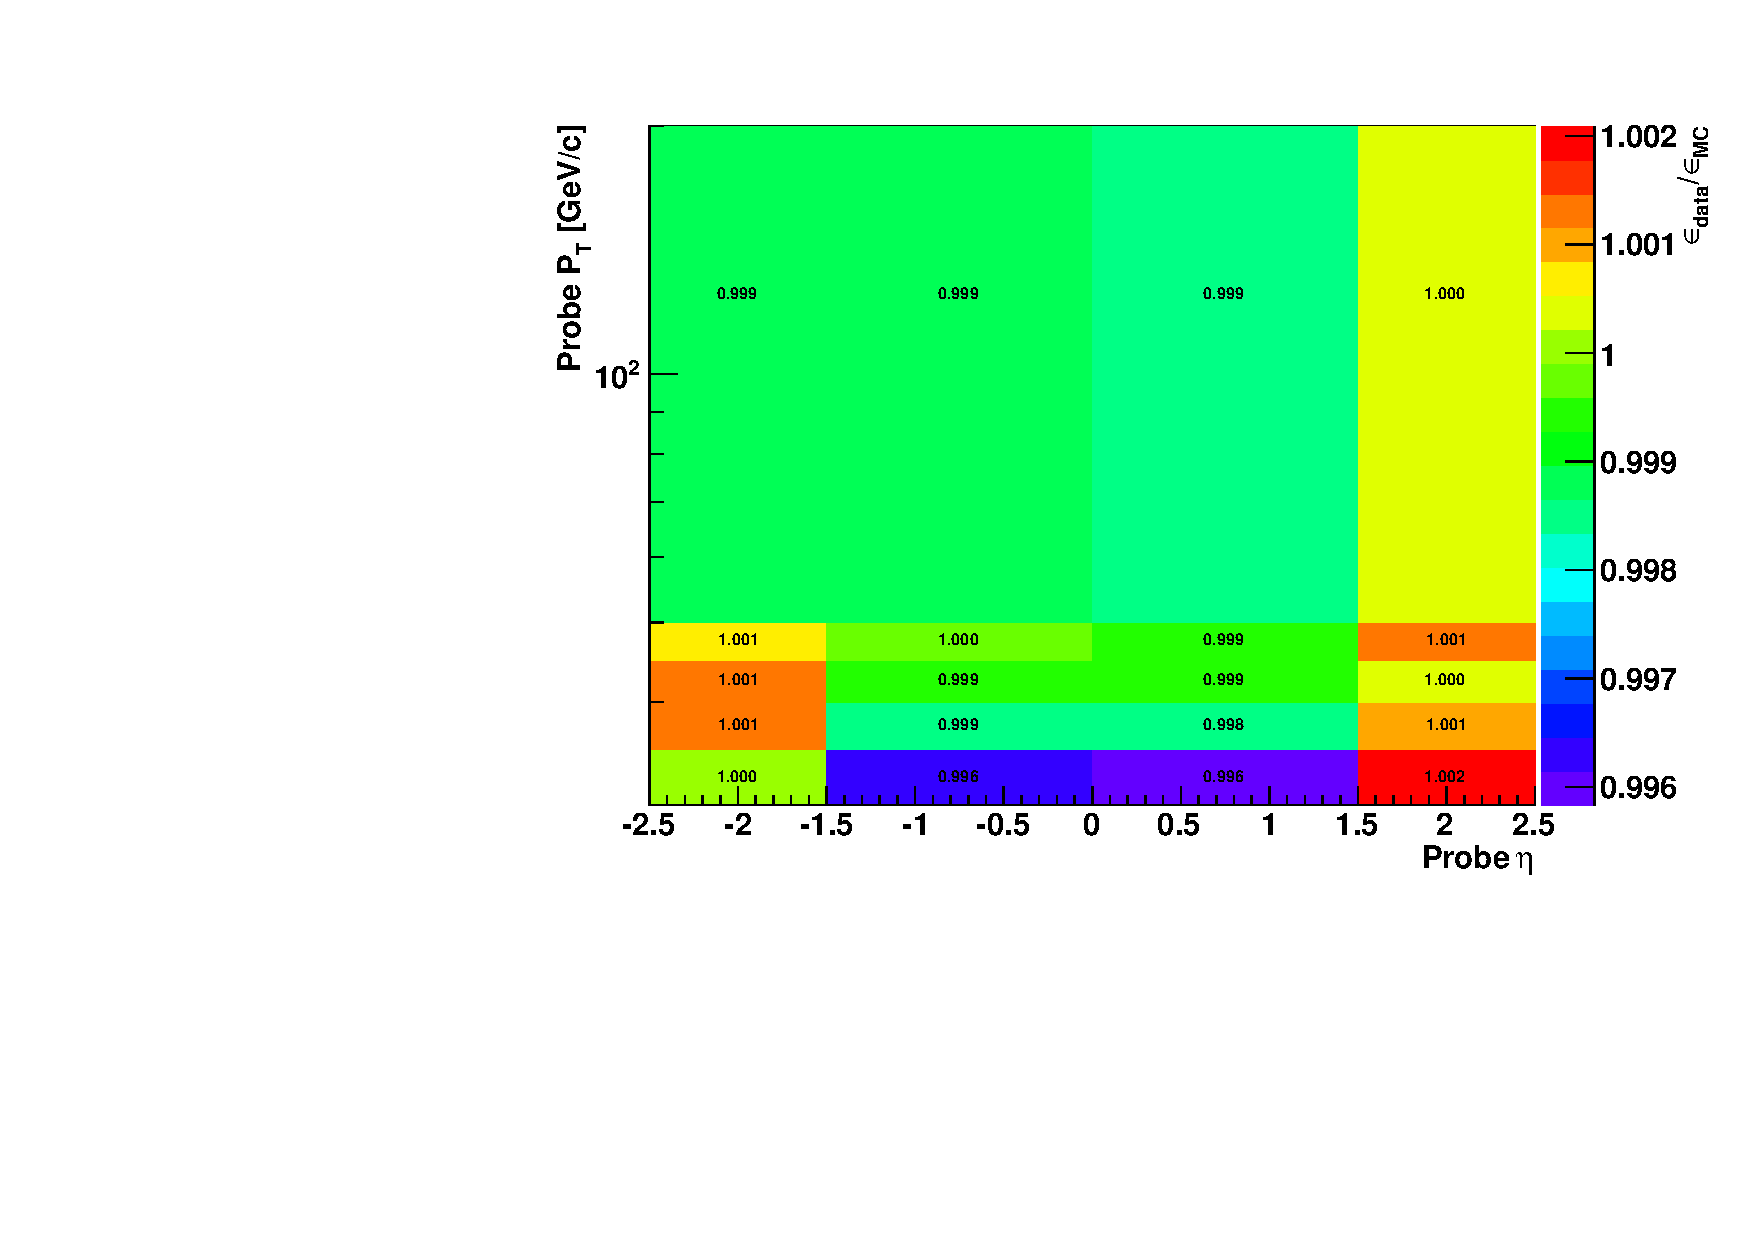
\includegraphics[width=0.32\textwidth]{figs/scaleFactor-Run2012ABC-SCToElectron.pdf}
  }
    \subfigure[]{
    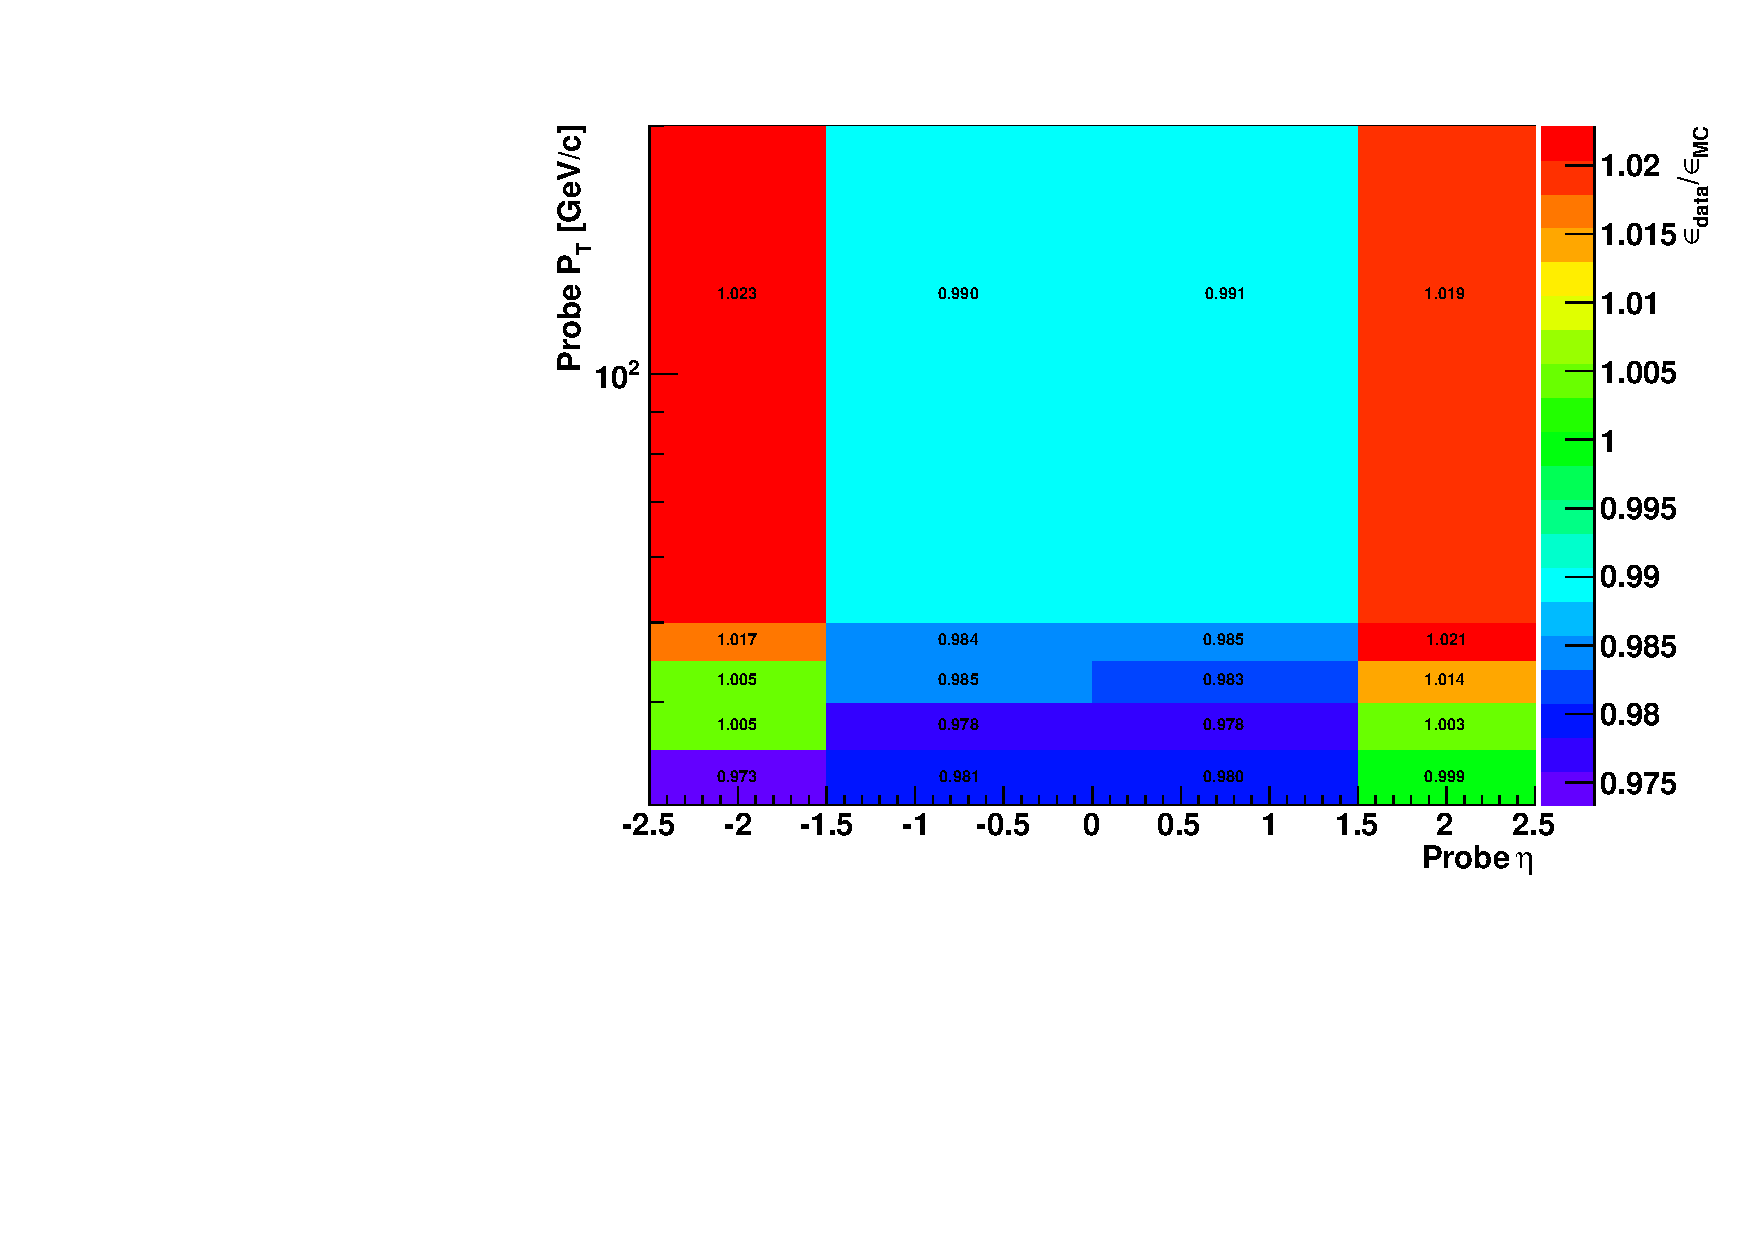
\includegraphics[width=0.32\textwidth]{figs/scaleFactor-Run2012ABC-GsfElectronToId.pdf}
  }
  \subfigure[]{
    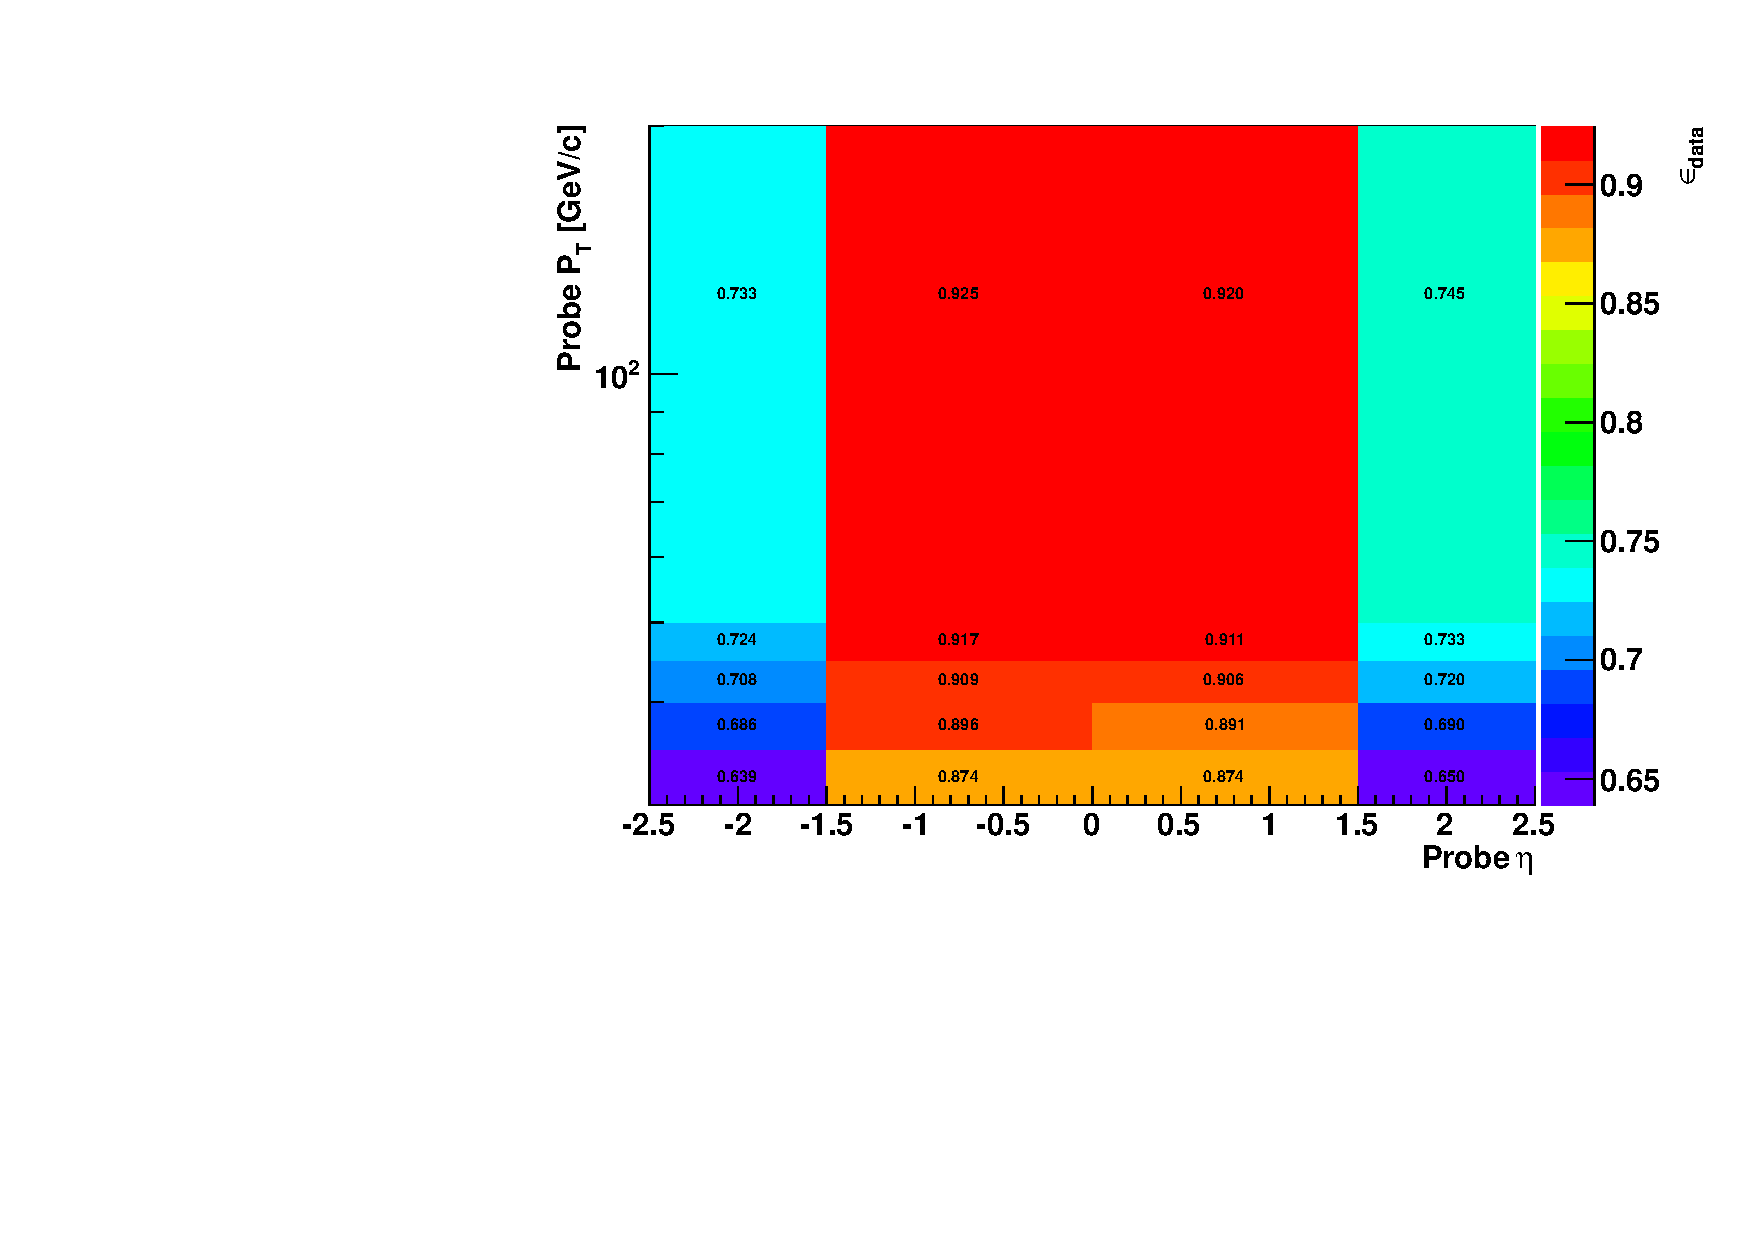
\includegraphics[width=0.32\textwidth]{figs/efficiency-Run2012ABC-WP80ToHLTEle.pdf}
  }
    \caption{Electron efficiency and data/MC scale factors for super-cluster to reconstructed electrons $\epsilon_{\textnormal{Reco}}$ (a),
    reconstructed to selected electrons $\epsilon_{\textnormal{Id}}$ (b) and selected to HLT electrons
      $\epsilon_{\textnormal{HLT}}$ (c).}
    \label{fig:eleEff}
  \end{center}
\end{figure}

\subsection{Muon efficiencies}\label{subsec:EffMu}

In the muon case, the reconstruction efficiency $\epsilon_{\textnormal{Reco}}$ describes the ability to reconstruct a Particle Flow muon starting with
a particle track and can be assumed to be one \cite{MUONPAS}. The identification efficiency $\epsilon_{\textnormal{Id}}$ gives an estimate for a
reconstructed muon to pass the offline selection criteria. It can be computed for both data and simulation and thus a scale factor,
the ratio of the two efficiencies, is derived. \\
The trigger efficiency $\epsilon_{\textnormal{HLT}}$  is the fraction of selected muons fulfilling the HLT requirements, and, since the HLT
requirement is dropped on the MC analysis, the efficiency computed on data is used directly to correct the MC event expectation.\\
The efficiency measurement is binned both in $\pt$ and $\eta$ of the probe muon covering the
relevant intervals (25, 30, 35, 40, 45, 50, 200)\GeVc in $\pt$ and (-2.1, -1.5, -1.0, -0.5, 0.0, 0.5, 1.0, 1.5, 2.1) in $\eta$. The resulting selection
and trigger efficiencies and scale factors are summarized in Table~\ref{tab:muonEff} and Figure~\ref{fig:muonEff}.

\begin{table}[htb]
\centering
\scalebox{0.70}{
  \begin{tabular}{|c|c|c|c|c|c|}
  \hline
  $p_{\textnormal{T,min}}$ & $p_{\textnormal{T,max}}$ & $\eta_{\textnormal{min}}$ & $\eta_{\textnormal{max}}$ & $\epsilon_{\textnormal{ID,data}}$/$\epsilon_{\textnormal{ID,mc}}$ & $\epsilon_{\textnormal{HLT,data}}$ \\
  $[\GeVc]$         & $[\GeVc]$         &                     &                     &                             &                               \\
  \hline
  \hline
  25 & 30 & -2.1 & -1.5 & 0.992 $\pm$ 0.003 & 0.766 $\pm$ 0.003 \\
  25 & 30 & -1.5 & -1 & 0.987 $\pm$ 0.003 & 0.822 $\pm$ 0.003 \\
  25 & 30 & -1 & -0.5 & 0.990 $\pm$ 0.003 & 0.914 $\pm$ 0.002 \\
  25 & 30 & -0.5 & 0 & 0.984 $\pm$ 0.003 & 0.920 $\pm$ 0.002 \\
  25 & 30 & 0 & 0.5 & 0.985 $\pm$ 0.003 & 0.924 $\pm$ 0.002 \\
  25 & 30 & 0.5 & 1 & 0.992 $\pm$ 0.003 & 0.913 $\pm$ 0.002 \\
  25 & 30 & 1 & 1.5 & 0.991 $\pm$ 0.003 & 0.802 $\pm$ 0.003 \\
  25 & 30 & 1.5 & 2.1 & 0.995 $\pm$ 0.002 & 0.814 $\pm$ 0.003 \\
  30 & 35 & -2.1 & -1.5 & 0.991 $\pm$ 0.002 & 0.785 $\pm$ 0.002 \\
  30 & 35 & -1.5 & -1 & 0.988 $\pm$ 0.002 & 0.829 $\pm$ 0.002 \\
  30 & 35 & -1 & -0.5 & 0.988 $\pm$ 0.002 & 0.921 $\pm$ 0.002 \\
  30 & 35 & -0.5 & 0 & 0.984 $\pm$ 0.002 & 0.930 $\pm$ 0.001 \\
  30 & 35 & 0 & 0.5 & 0.985 $\pm$ 0.002 & 0.935 $\pm$ 0.001 \\
  30 & 35 & 0.5 & 1 & 0.990 $\pm$ 0.002 & 0.922 $\pm$ 0.002 \\
  30 & 35 & 1 & 1.5 & 0.987 $\pm$ 0.002 & 0.807 $\pm$ 0.002 \\
  30 & 35 & 1.5 & 2.1 & 0.995 $\pm$ 0.002 & 0.833 $\pm$ 0.002 \\
  35 & 40 & -2.1 & -1.5 & 0.992 $\pm$ 0.002 & 0.793 $\pm$ 0.002 \\
  35 & 40 & -1.5 & -1 & 0.987 $\pm$ 0.002 & 0.832 $\pm$ 0.002 \\
  35 & 40 & -1 & -0.5 & 0.991 $\pm$ 0.002 & 0.926 $\pm$ 0.001 \\
  35 & 40 & -0.5 & 0 & 0.986 $\pm$ 0.002 & 0.935 $\pm$ 0.001 \\
  35 & 40 & 0 & 0.5 & 0.986 $\pm$ 0.002 & 0.940 $\pm$ 0.001 \\
  35 & 40 & 0.5 & 1 & 0.991 $\pm$ 0.002 & 0.925 $\pm$ 0.001 \\
  35 & 40 & 1 & 1.5 & 0.989 $\pm$ 0.002 & 0.812 $\pm$ 0.002 \\
  35 & 40 & 1.5 & 2.1 & 0.994 $\pm$ 0.002 & 0.837 $\pm$ 0.002 \\
  40 & 45 & -2.1 & -1.5 & 0.994 $\pm$ 0.002 & 0.800 $\pm$ 0.002 \\
  40 & 45 & -1.5 & -1 & 0.987 $\pm$ 0.001 & 0.837 $\pm$ 0.002 \\
  40 & 45 & -1 & -0.5 & 0.992 $\pm$ 0.001 & 0.927 $\pm$ 0.001 \\
  40 & 45 & -0.5 & 0 & 0.986 $\pm$ 0.001 & 0.940 $\pm$ 0.001 \\
  40 & 45 & 0 & 0.5 & 0.987 $\pm$ 0.001 & 0.944 $\pm$ 0.001 \\
  40 & 45 & 0.5 & 1 & 0.991 $\pm$ 0.001 & 0.928 $\pm$ 0.001 \\
  40 & 45 & 1 & 1.5 & 0.991 $\pm$ 0.001 & 0.817 $\pm$ 0.002 \\
  40 & 45 & 1.5 & 2.1 & 0.996 $\pm$ 0.001 & 0.844 $\pm$ 0.002 \\
  45 & 50 & -2.1 & -1.5 & 0.993 $\pm$ 0.002 & 0.807 $\pm$ 0.002 \\
  45 & 50 & -1.5 & -1 & 0.987 $\pm$ 0.002 & 0.840 $\pm$ 0.002 \\
  45 & 50 & -1 & -0.5 & 0.990 $\pm$ 0.001 & 0.931 $\pm$ 0.001 \\
  45 & 50 & -0.5 & 0 & 0.988 $\pm$ 0.002 & 0.941 $\pm$ 0.001 \\
  45 & 50 & 0 & 0.5 & 0.987 $\pm$ 0.002 & 0.947 $\pm$ 0.001 \\
  45 & 50 & 0.5 & 1 & 0.992 $\pm$ 0.001 & 0.930 $\pm$ 0.001 \\
  45 & 50 & 1 & 1.5 & 0.991 $\pm$ 0.002 & 0.821 $\pm$ 0.002 \\
  45 & 50 & 1.5 & 2.1 & 0.995 $\pm$ 0.002 & 0.851 $\pm$ 0.002 \\
  50 & 200 & -2.1 & -1.5 & 0.991 $\pm$ 0.002 & 0.809 $\pm$ 0.002 \\
  50 & 200 & -1.5 & -1 & 0.987 $\pm$ 0.002 & 0.842 $\pm$ 0.002 \\
  50 & 200 & -1 & -0.5 & 0.992 $\pm$ 0.002 & 0.931 $\pm$ 0.001 \\
  50 & 200 & -0.5 & 0 & 0.987 $\pm$ 0.002 & 0.944 $\pm$ 0.001 \\
  50 & 200 & 0 & 0.5 & 0.989 $\pm$ 0.002 & 0.946 $\pm$ 0.001 \\
  50 & 200 & 0.5 & 1 & 0.992 $\pm$ 0.002 & 0.932 $\pm$ 0.001 \\
  50 & 200 & 1 & 1.5 & 0.993 $\pm$ 0.002 & 0.824 $\pm$ 0.002 \\
  50 & 200 & 1.5 & 2.1 & 0.996 $\pm$ 0.002 & 0.854 $\pm$ 0.002 \\
  \hline
  \end{tabular}}
\caption{Muon selection scale factors and HLT efficiencies. The errors are statistical only.}
\label{tab:muonEff}
\end{table}


\begin{figure}[t]
  \begin{center}
    \subfigure[]{
    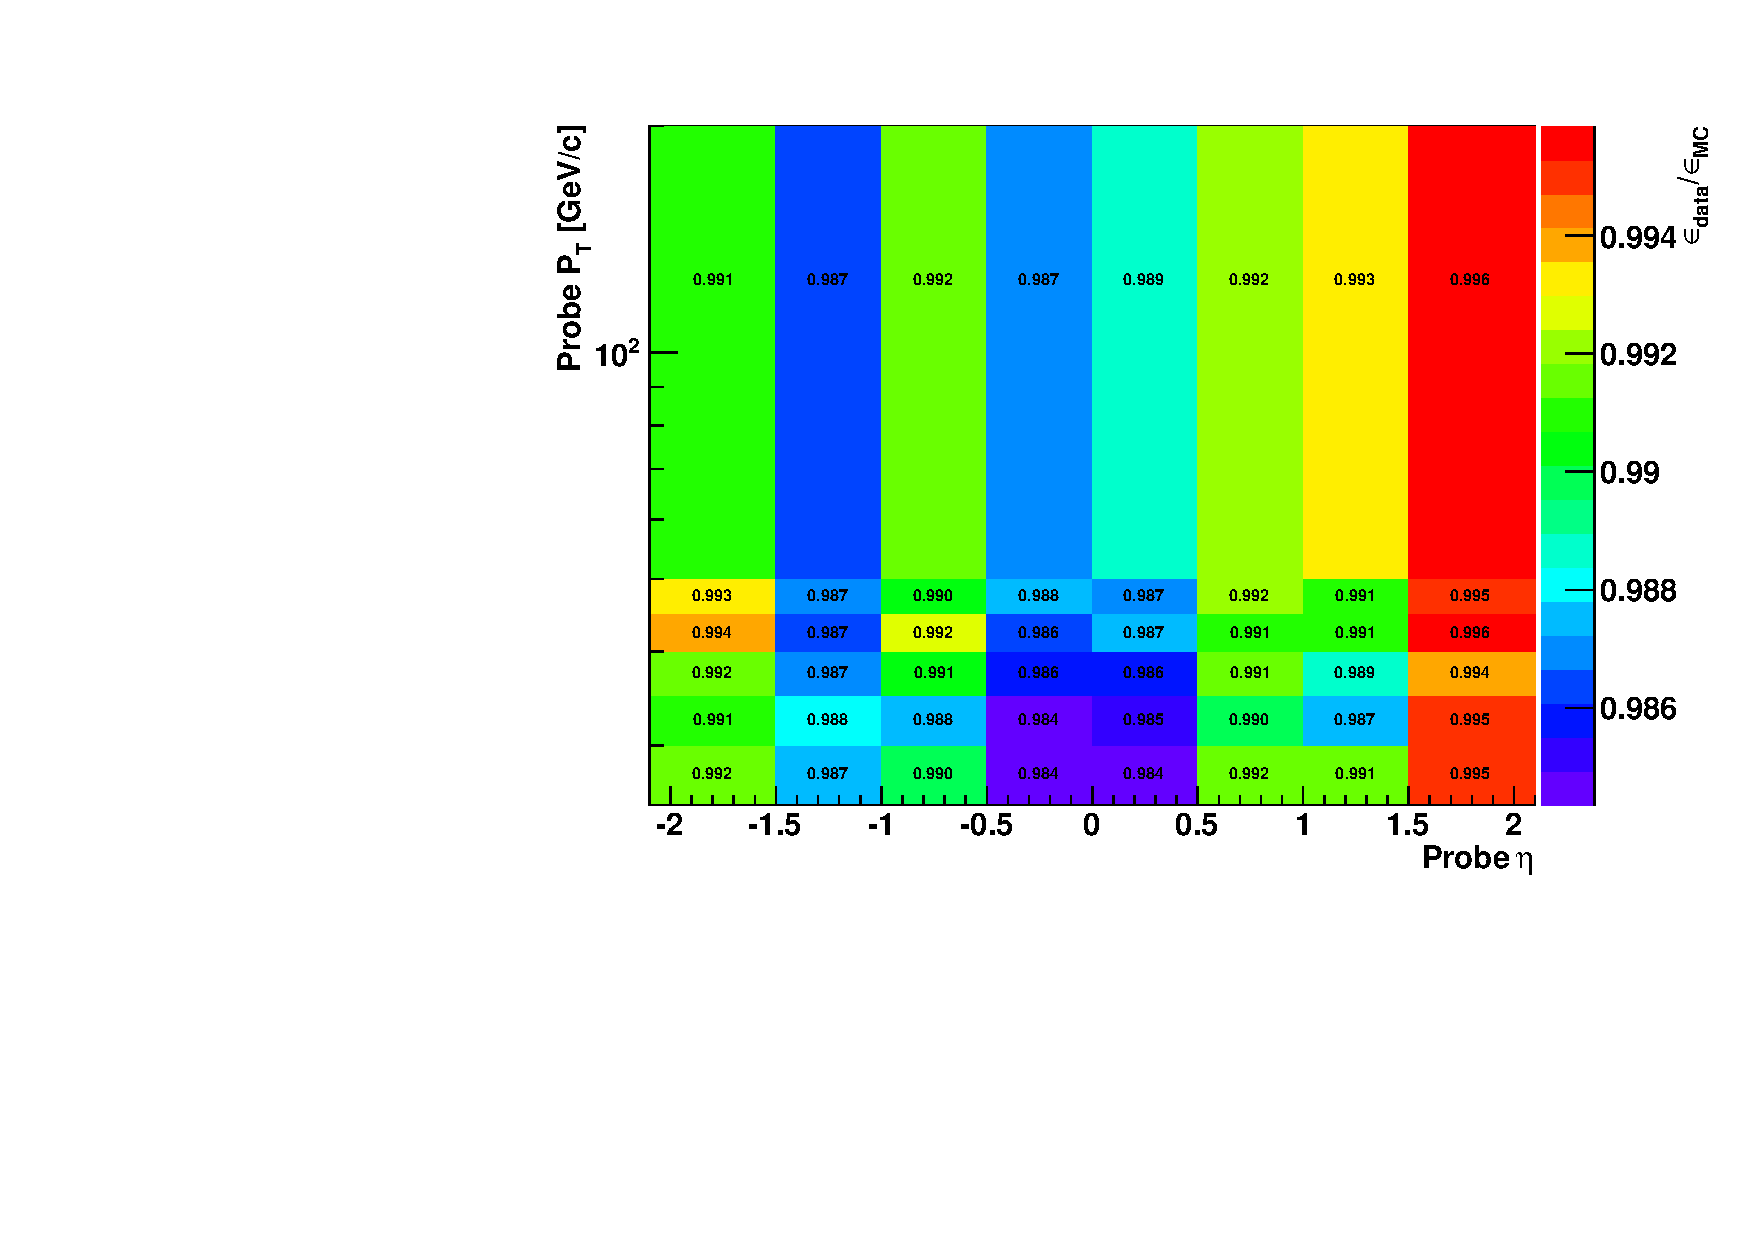
\includegraphics[width=0.47\textwidth]{figs/scaleFactor-Run2012ABC-RecoToIso.pdf}
  }
  \subfigure[]{
    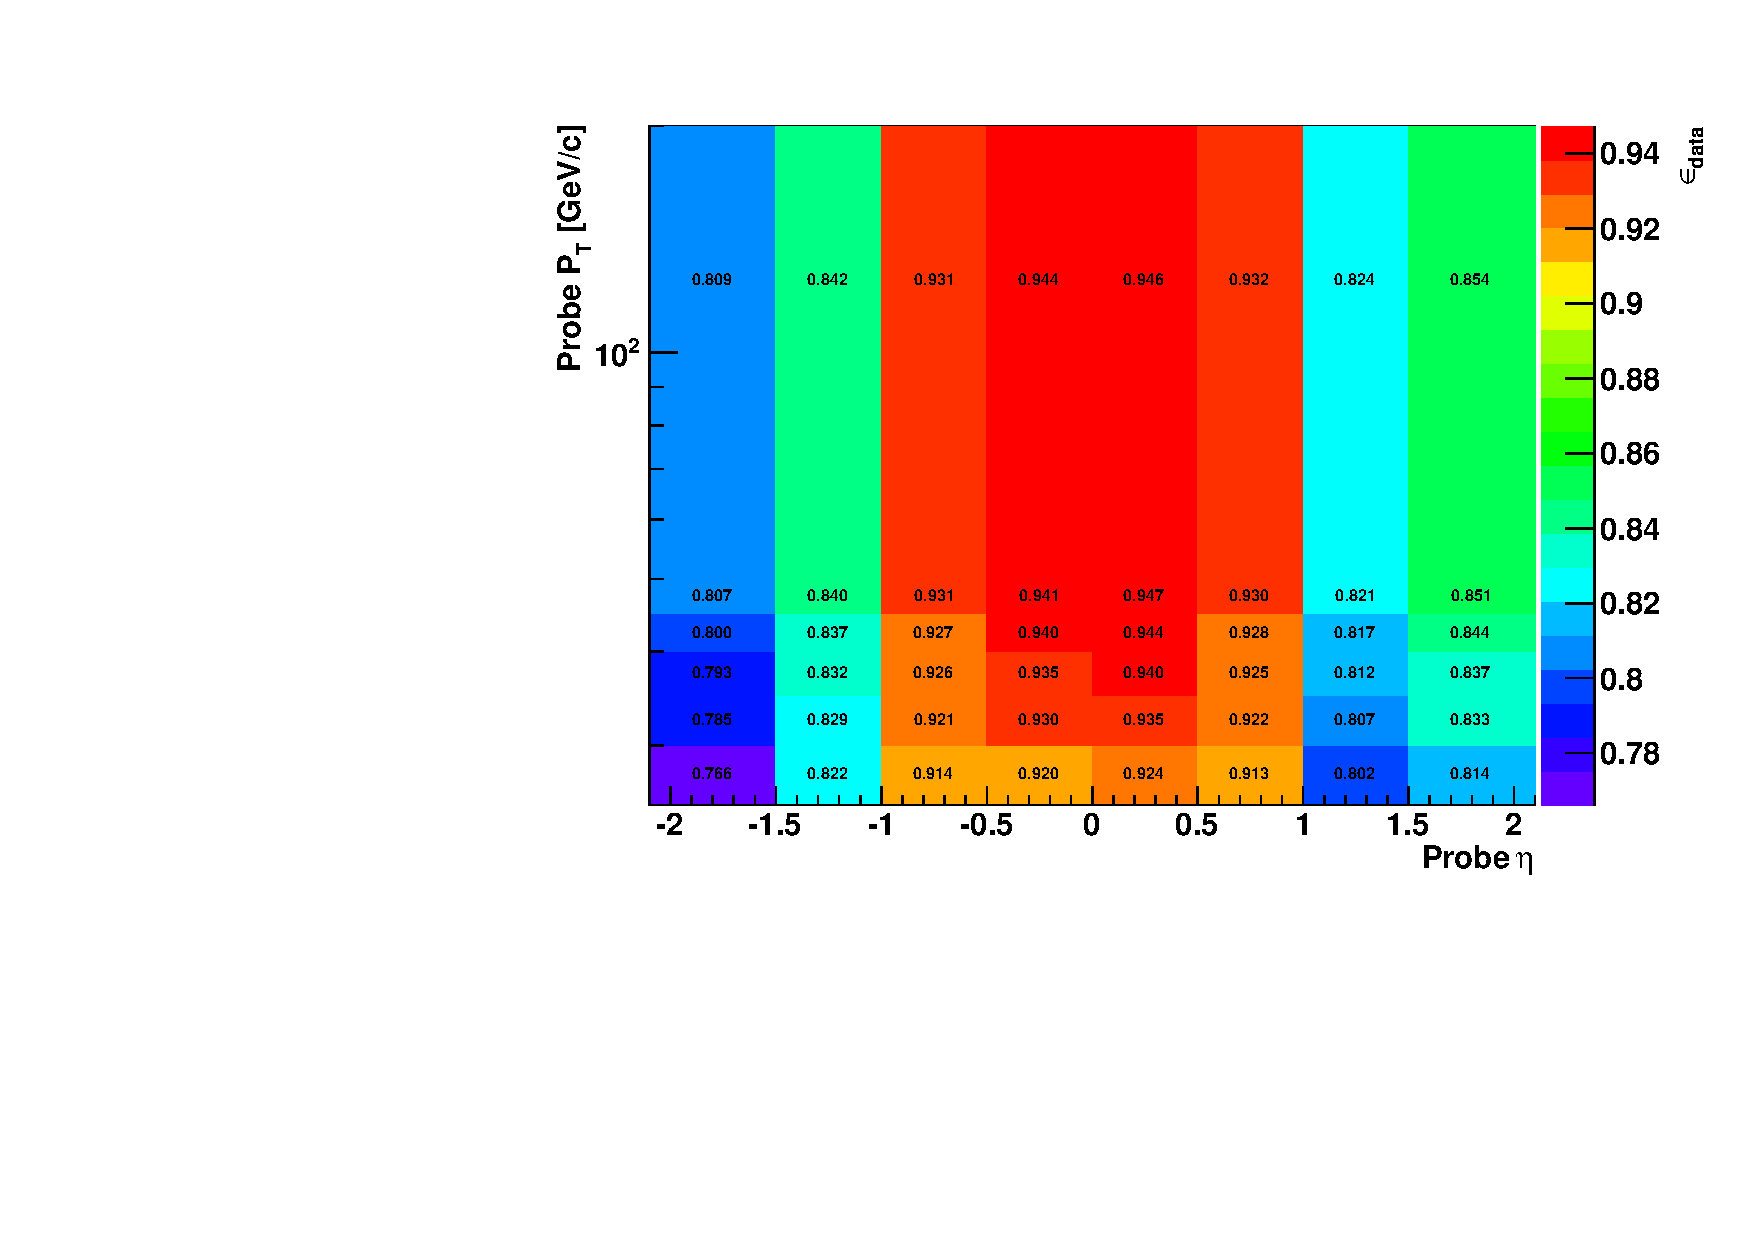
\includegraphics[width=0.47\textwidth]{figs/efficiency-Run2012ABC-IsoToIsoMuHLT.pdf}
  }
    \caption{Muon scale factors for reconstructed to selected muons $\epsilon_{\textnormal{ID,data}}$/$\epsilon_{\textnormal{ID,mc}}$ (a) and
    efficiency for selected to HLT muons $\epsilon_{\textnormal{HLT,data}}$ (b).}
    \label{fig:muonEff}
  \end{center}
\end{figure}



%%%%%%%%%%%%%%%%%%%%%%%%%%%%%%%%%%%%%%%%%%%%%%%%%%%%%%%%%%%%%%%%%%%%%%%%%%
%%%%%%%%%%%%%%%%%%%%%%%%%%%%%%%%%%%%%%%%%%%%%%%%%%%%%%%%%%%%%%%%%%%%%%%%%%
\clearpage{}
\section{Results}
\label{sec:results}
% ---- ---- ---- ---- ---- ---- ---- ---- ---- ---- ---- ---- ---- ---- ----
\par
The well-known formula for the extraction of  a cross section is:
\begin{equation}
\label{eq:xsec}
 \sigma = \frac{N^{\text{Sig}}}
               { A \, \epsilon \, {\cal{L}} }
\end{equation}
where $N^{\text{Sig}}$ is the number of extracted signal events,
$A$ is the signal acceptance corrected for the branching fraction,
$\epsilon$ is the efficiency for all requirements on 
the event selection, and ${\cal{L}}$ is the integrated luminosity.
Using the number of signal diboson events from 
table~\ref{table:FitTotalsAndComparisons} and efficiency $\times$ 
acceptance values from table~\ref{tab:signals}, we obtain the 
WW+WZ cross section values for each disjoint sub-sample as shown in 
table~\ref{tab:measuredCrossSection}
%%%%%%%%%%%%%%%%%%%%%%%%%%%%%
\begin{table}[h]
\begin{center}
  \begin{tabular}{l c}
    \hline  \hline
    Event category &  Measured cross section\\
    \hline
    $\mu jj$        &    $73.41 \pm 15.07$  pb\\
    $ejj$           &    $60.14 \pm 21.50$  pb\\   \hline 
    $\mu jj$,b-tag  &    $76.85 \pm 60.68$  pb\\
    $ejj$,b-tag     &    $22.71 \pm 49.27$  pb\\   \hline 
    Theory prediction~\cite{Campbell:2011bn} &  $65.6 \pm 2.2$ pb\\
    \hline  \hline
  \end{tabular}
\end{center}
\caption{\label{tab:measuredCrossSection}
The measured values of the sum of WW and WZ cross section in each disjoint sub-sample. 
The uncertainties include both statistical and systematic.}
\end{table}
%%%%%%%%%%%%%%%%%%%%%%%%%%%%%

Combining all four channels, we obtain:

WW+WZ cross section = 66.70 $\pm$ 11.74 pb.\\
[Breaking down the uncertainties: 66.70 $\pm$ 8.08 (stat) $\pm$ 8.52 (syst) pb]


We produce combined plots for electrons and muons in
Figs~\ref{fig:combinedNoBtag} and~\ref{fig:combinedWithBtag} for no $b$
tags and with $b$ tags, respectively.

\begin{figure}
\begin{center}
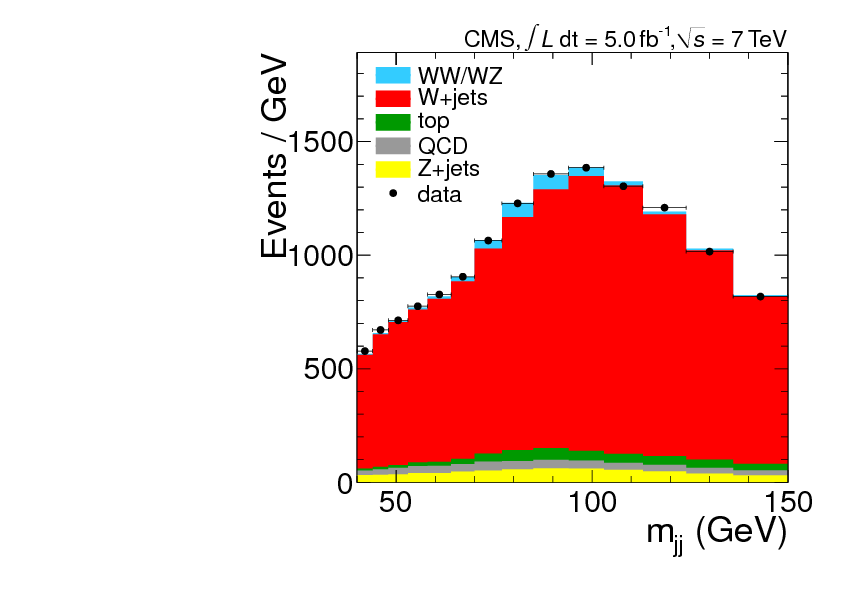
\includegraphics[width=0.45\textwidth]{figs/mjjfit_2jetsample/Diboson_Stacked_combined}
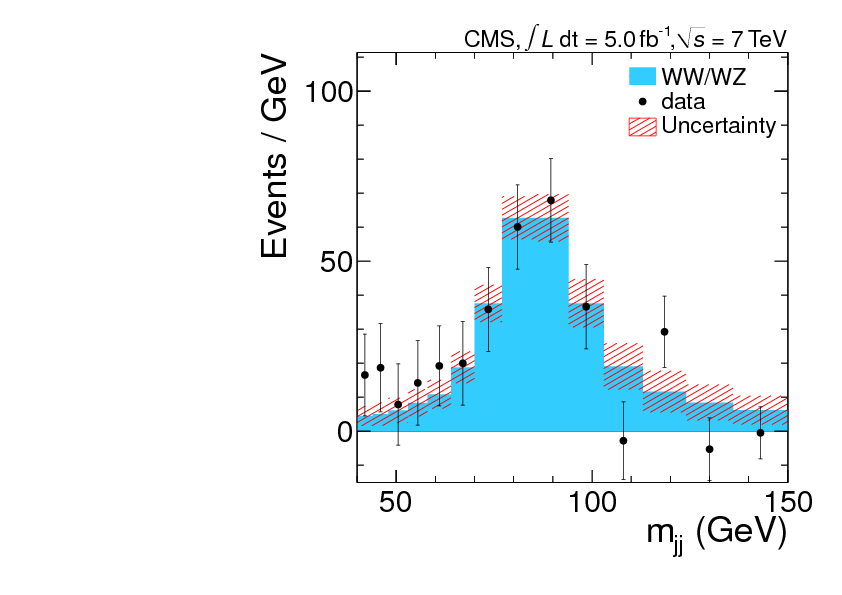
\includegraphics[width=0.45\textwidth]{figs/mjjfit_2jetsample/Diboson_Subtracted_combined}
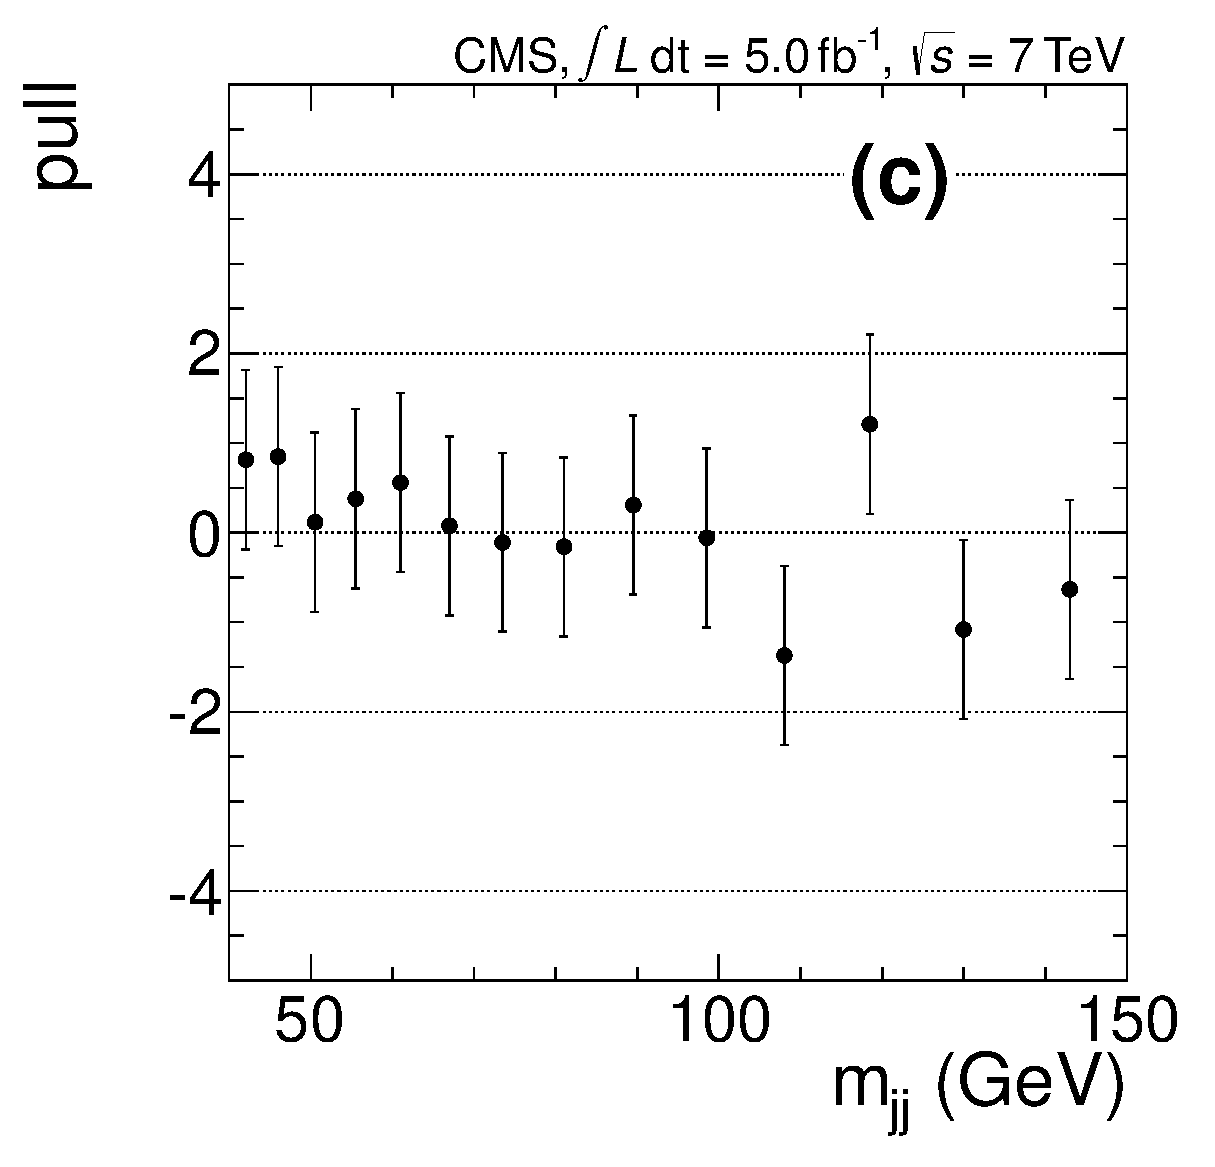
\includegraphics[width=0.45\textwidth]{figs/mjjfit_2jetsample/Diboson_Pull_combined}
\end{center}
\caption{Combined results of both muons and electrons without btags}
\label{fig:combinedNoBtag}
\end{figure}

\begin{figure}
\begin{center}
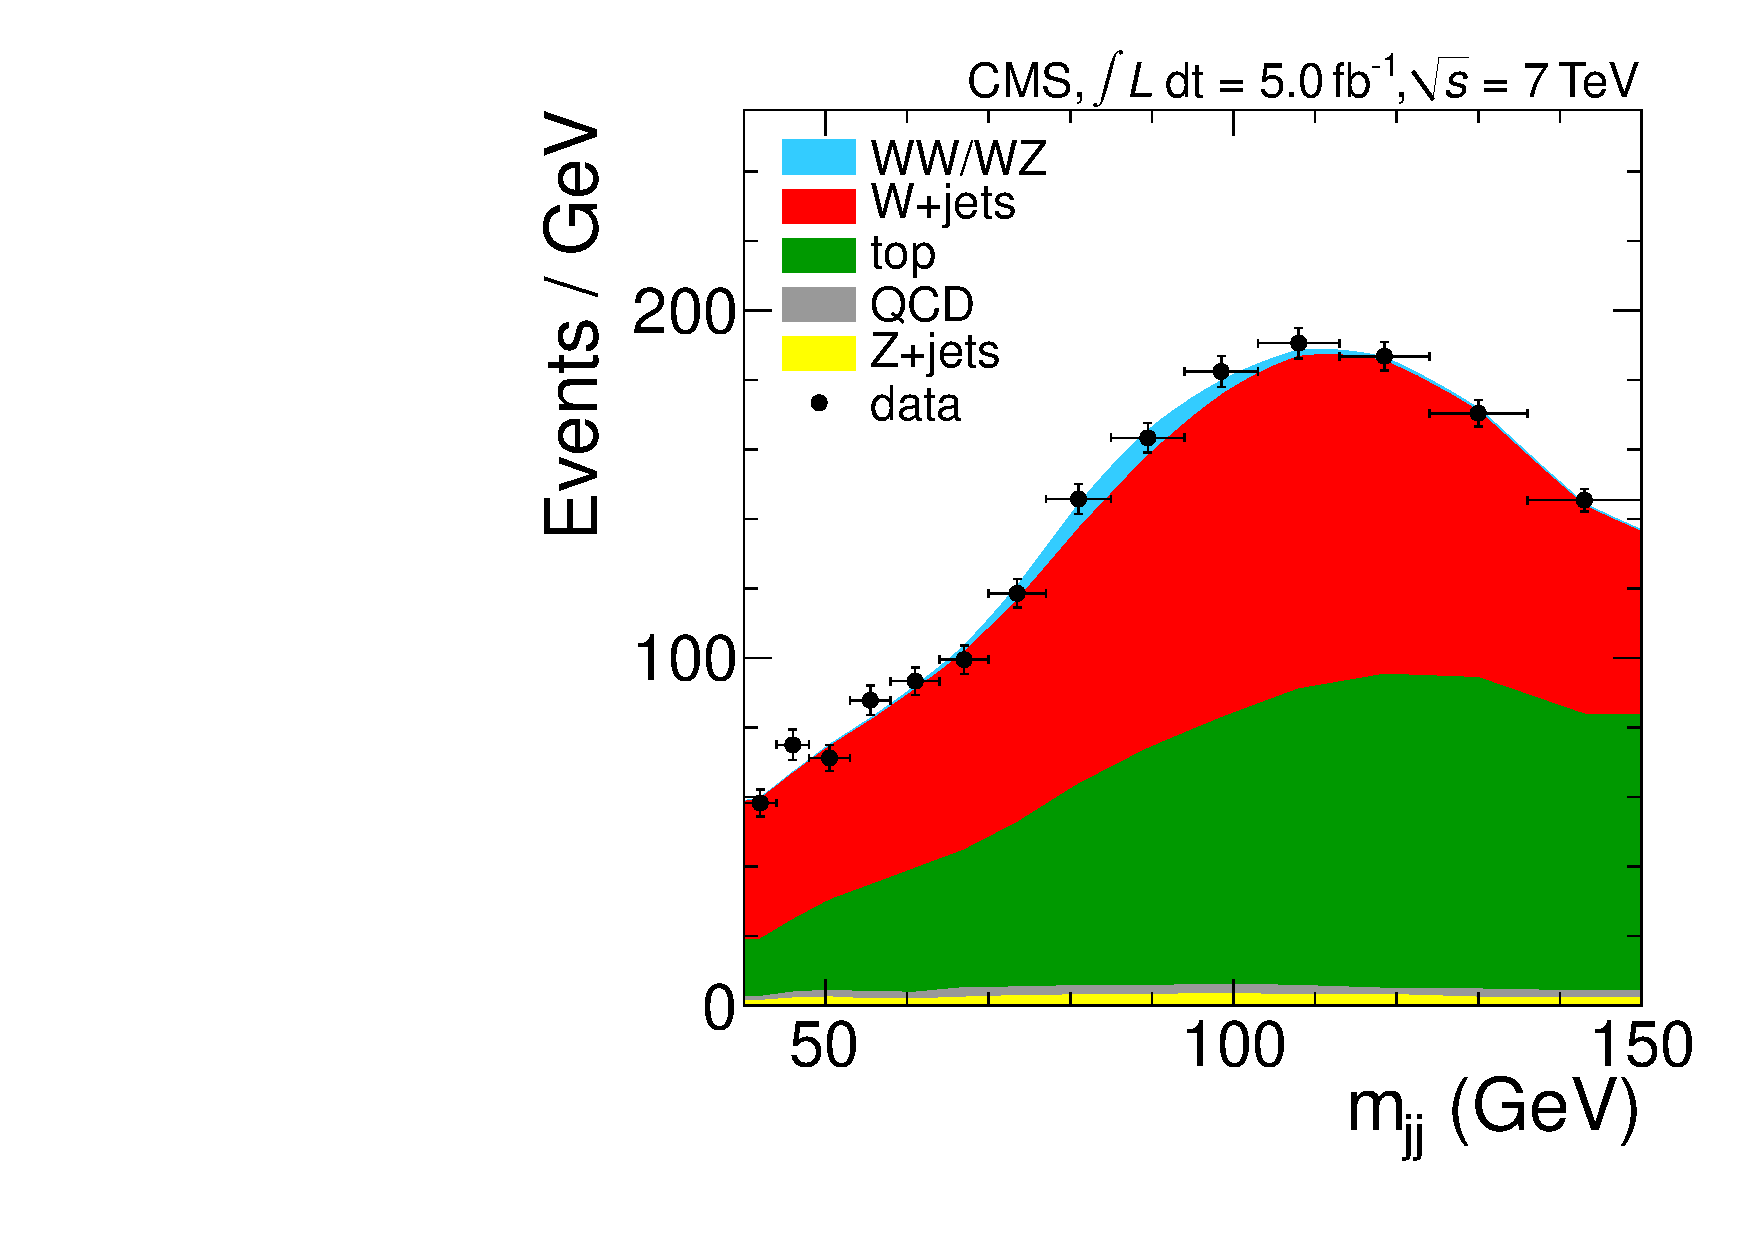
\includegraphics[width=0.45\textwidth]{figs/mjjfit_2jetsample/Diboson_btag_Stacked_combined}
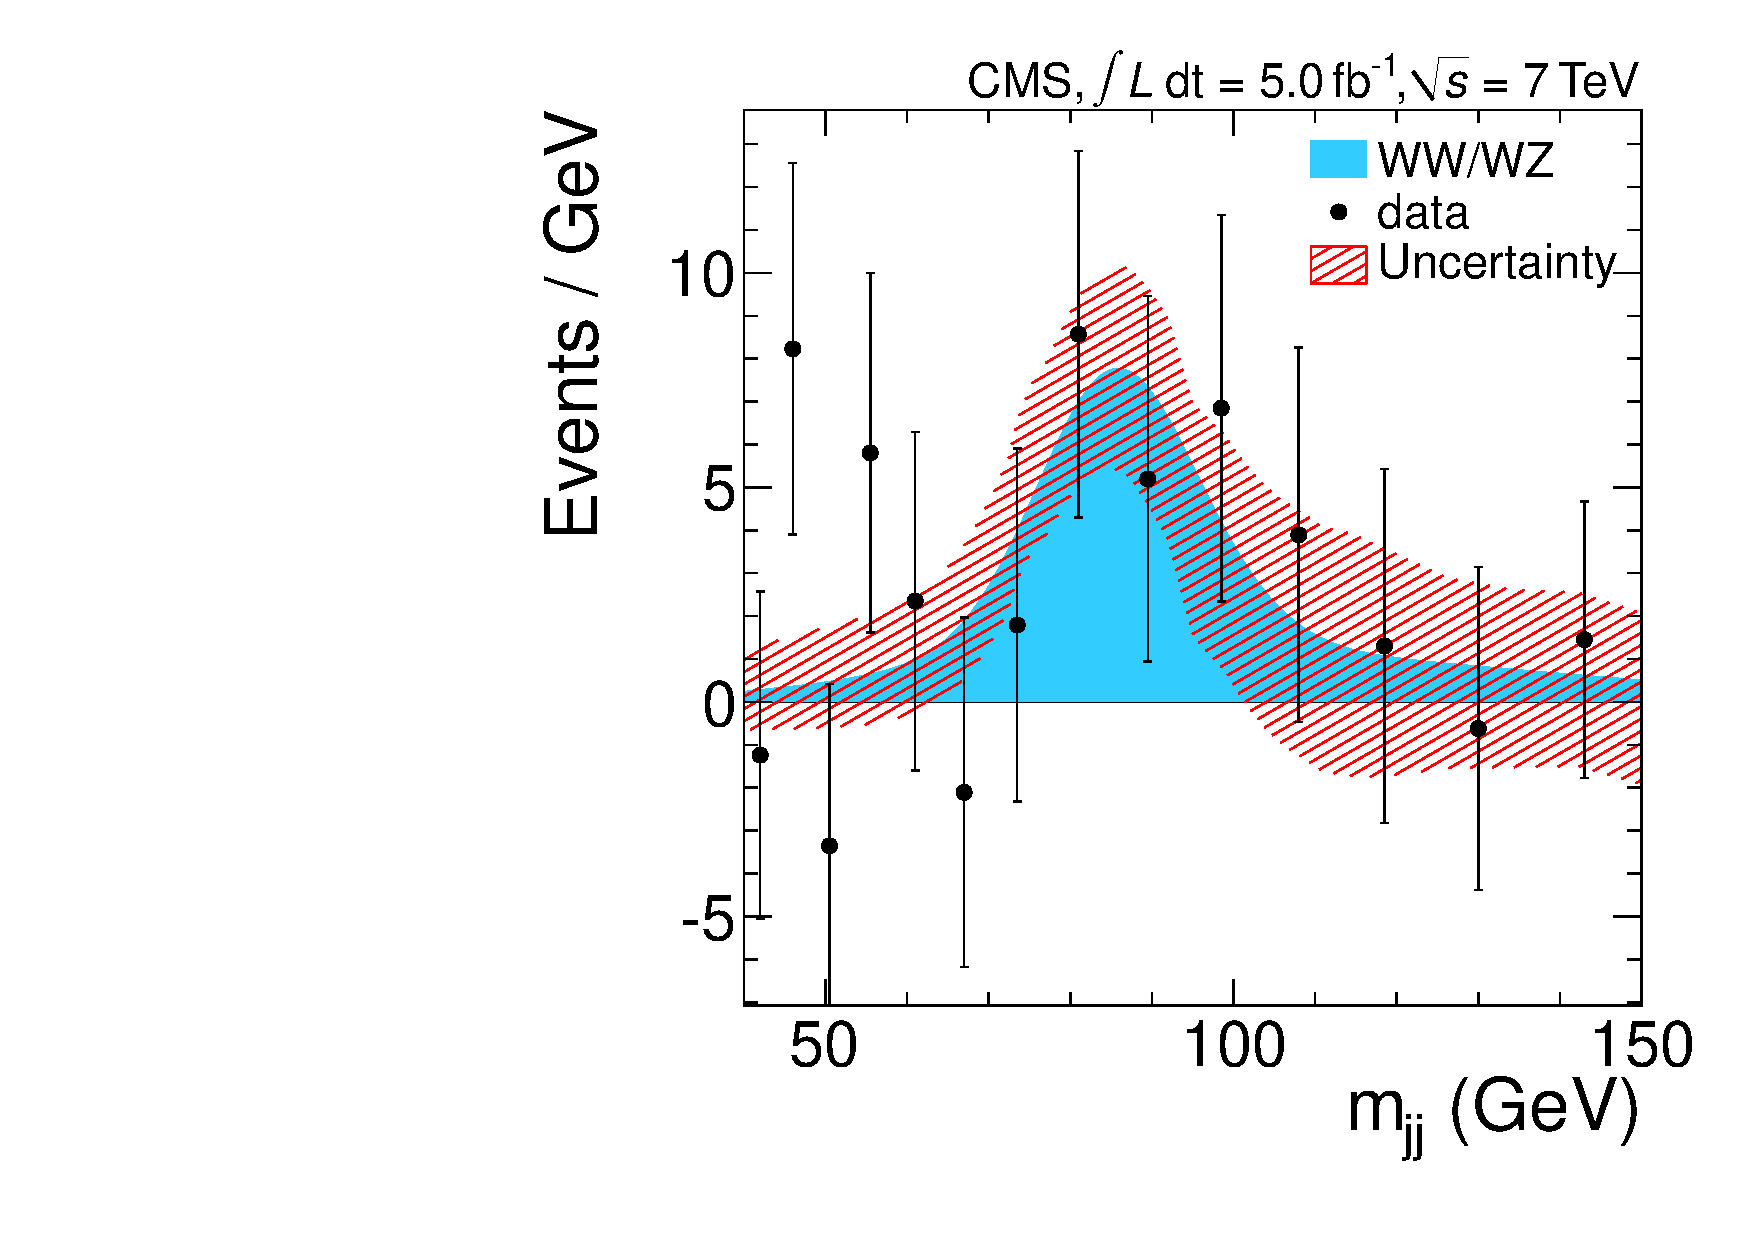
\includegraphics[width=0.45\textwidth]{figs/mjjfit_2jetsample/Diboson_btag_Subtracted_combined}
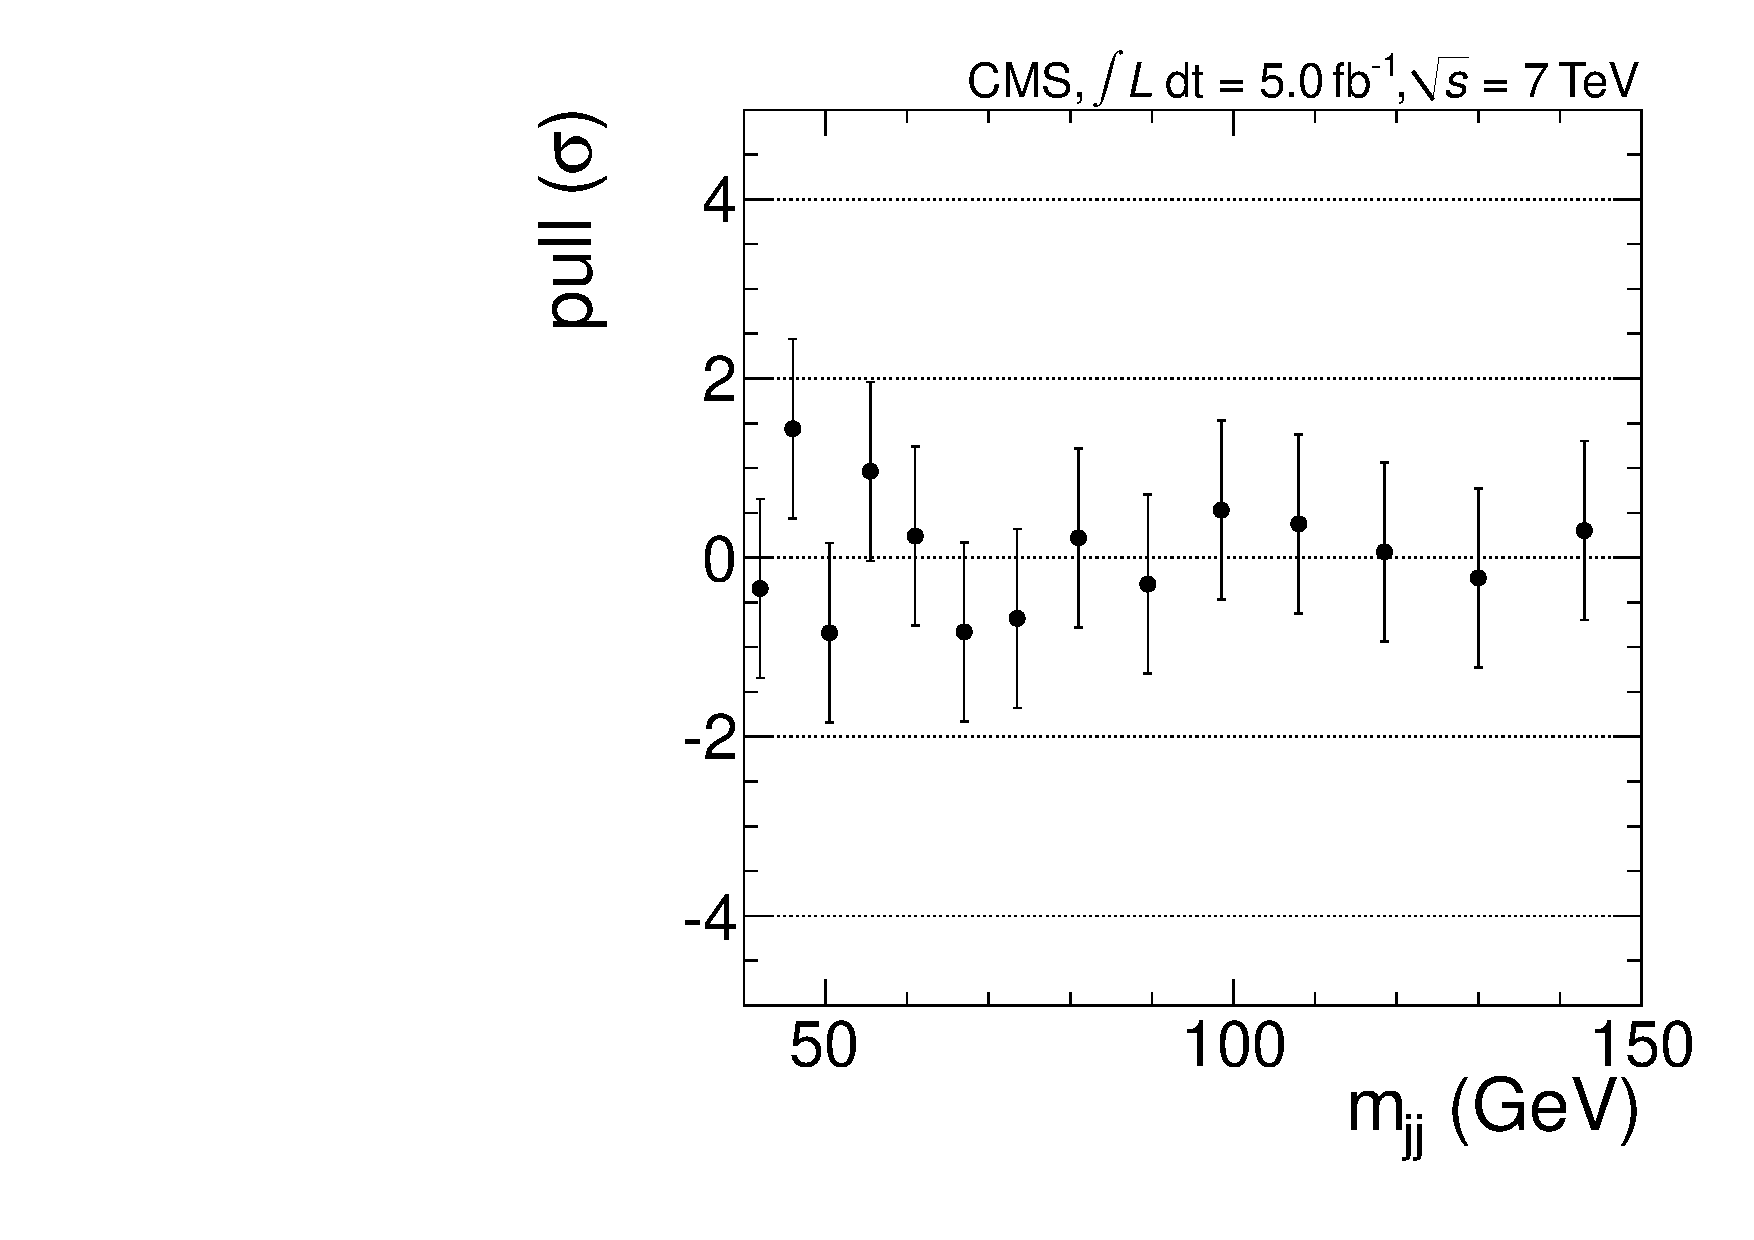
\includegraphics[width=0.45\textwidth]{figs/mjjfit_2jetsample/Diboson_btag_Pull_combined}
\end{center}
\caption{Combined results of both muons and electrons with btags}
\label{fig:combinedWithBtag}
\end{figure}


\subsection{Results including only non b-tag categories}
\label{sec:results2ch}
% ---- ---- ---- ---- ---- ---- ---- ---- ---- ---- ---- ---- ---- ---- ----
Including only non b-tag (both muon and electron) categories, we 
observe 2682 $\pm$ 339 (stat) $\pm$ 357 (syst) WW+WZ events, 
in agreement with the Standard Model expectation. 
This corresponds to a significance of $8.8~\sigma$ 
($7.8~\sigma$ in muon data and $4.4~\sigma$ in electron data) 
when computed using a simple likelihood 
ratio where the nuisance parameters are fixed to their nominal fit 
values in case of the null hypothesis. 
Using the profile likelihood ratio, where the nuisance parameters are 
allowed to vary also for the null hypothesis, the significance 
becomes $4.34~\sigma$ ($4.31~\sigma$ in muon data 
and $1.60~\sigma$ in electron data).


Combining results of muon and electron non b-tag categories, we obtain
the following result for cross section:
$\sigma = 68.89 \pm 8.71 \text{(stat)} \pm 9.70 \text{(syst)}  \pm 1.52 \text{(lumi)}$~pb, 
which is in agreement with the NLO prediction 
$65.6 \pm 2.2$~pb that includes $gg\to\text{WW}$ contribution.

\section{Conclusions}
\label{sec:conclusions}
We have studied the electroweak production 
of two heavy gauge bosons  in events 
with a leptonically decaying W boson and exactly two jets.
The analyzed dataset 
corresponds to an integrated luminosity of 5.0~fb${}^{-1}$ at 
$\sqrt{s} = 7$~TeV collected by the CMS detector at the Large Hadron Collider.
With the kinematic requirements imposed in the analysis, we 
observe 2979 $\pm$ 361 (stat) $\pm$ 402 (syst) WW+WZ events, 
in agreement with the Standard Model expectation. 
The measured value of the sum of WW and WZ cross sections is 
66.7 $\pm$ 8.1 (stat) $\pm$ 8.5 (syst) pb, consistent 
with the standard model prediction of 65.6~pb. 
This is the first observation of diboson events in 
the semi-leptonic final state in a pp collider.
We derive limits on anomalous triple gauge couplings  
using the $p_T$ distribution of the dijet system: 
$ -0.038 < \lambda_Z < 0.030$, 
$ -0.111 < \Delta{\kappa_\gamma} < 0.142$.
These limits are the most stringent at a hadron collider to-date 
and are approaching the sensitivity of combined LEP measurements.


We congratulate our colleagues in the CERN accelerator departments for the excellent performance of the LHC and thank the 
technical and administrative staffs at CERN and at other CMS institutes for their contributions to the success of the CMS 
effort. In addition, we gratefully acknowledge the computing centres and personnel of the Worldwide LHC Computing Grid for 
delivering so effectively the computing infrastructure essential to our analyses. Finally, we acknowledge the enduring support 
for the construction and operation of the LHC and the CMS detector provided by the following funding agencies: BMWF and FWF 
(Austria); FNRS and FWO (Belgium); CNPq, CAPES, FAPERJ, and FAPESP (Brazil); MES (Bulgaria); CERN; CAS, MoST, and NSFC (China); 
COLCIENCIAS (Colombia); MSES and CSF (Croatia); RPF (Cyprus); MoER, SF0690030s09 and ERDF (Estonia); Academy of Finland, MEC, 
and HIP (Finland); CEA and CNRS/IN2P3 (France); BMBF, DFG, and HGF (Germany); GSRT (Greece); OTKA and NIH (Hungary); DAE and 
DST (India); IPM (Iran); SFI (Ireland); INFN (Italy); NRF and WCU (Republic of Korea); LAS (Lithuania); MOE and UM (Malaysia); 
CINVESTAV, CONACYT, SEP, and UASLP-FAI (Mexico); MBIE (New Zealand); PAEC (Pakistan); MSHE and NSC (Poland); FCT (Portugal); 
JINR (Dubna); MON, RosAtom, RAS and RFBR (Russia); MESTD (Serbia); SEIDI and CPAN (Spain); Swiss Funding Agencies 
(Switzerland); NSC (Taipei); ThEPCenter, IPST, STAR and NSTDA (Thailand); TUBITAK and TAEK (Turkey); NASU (Ukraine); STFC 
(United Kingdom); DOE and NSF (USA).
 
Individuals have received support from the Marie-Curie programme and the European Research Council and EPLANET (European 
Union); the Leventis Foundation; the A. P. Sloan Foundation; the Alexander von Humboldt Foundation; the Belgian Federal Science 
Policy Office; the Fonds pour la Formation \`a la Recherche dans l'Industrie et dans l'Agriculture (FRIA-Belgium); the 
Agentschap voor Innovatie door Wetenschap en Technologie (IWT-Belgium); the Ministry of Education, Youth and Sports (MEYS) of 
Czech Republic; the Council of Science and Industrial Research, India; the Compagnia di San Paolo (Torino); the HOMING PLUS 
programme of Foundation for Polish Science, cofinanced by EU, Regional Development Fund; and the Thalis and Aristeia programmes 
cofinanced by EU-ESF and the Greek NSRF.
 

\clearpage

%% **DO NOT REMOVE BIBLIOGRAPHY**
\bibliography{auto_generated}   % will be created by the tdr script.

%%% DO NOT ADD \end{document}!

